%% Template for a scientific paper by Samuel Pawel
%% Last modification: 17. December 2020
\documentclass[a4paper, 11pt]{article}
\usepackage{alltt}
\usepackage[T1]{fontenc}
\usepackage[utf8]{inputenc}
\usepackage[english]{babel}
\usepackage{graphics}
\usepackage[dvipsnames]{xcolor}
\usepackage{amsmath, amssymb}
\usepackage{textcomp}
\usepackage{sourcesanspro} % use source sans pro as sans serif font
\usepackage[sc]{mathpazo}
\usepackage{times}
\usepackage{doi} % automatic doi-links
\usepackage[round]{natbib} % bibliography
\usepackage{multirow} % multi rows and columns for tables
\usepackage{longtable} % tables that span several pages
\usepackage{booktabs} % nicer tables
\usepackage[title]{appendix} % better appendices
\usepackage{nameref} % reference appendices with names
\usepackage[onehalfspacing]{setspace}
\usepackage[labelfont=bf,font=small]{caption}
\usepackage{pdfpages}
\usepackage{pdflscape}

% tikz for figure
\usepackage{tikz}
\usetikzlibrary{positioning, arrows}
\tikzset{
  % Define standard arrow tip
  >=stealth',
  % Define style for boxes
  punkt/.style={
    rectangle,
    rounded corners,
    draw=black, very thick,
    text width=6.5em,
    minimum height=10em,
    minimum width = 10em
    text centered},
  % Define arrow style
  pil/.style={
    ->,
    thick,
    shorten <=2pt,
    shorten >=2pt,}
}
\definecolor{lightg}{RGB}{230,230,230}

%% margins
%% ----------------------------------------------------------------------------
\usepackage{geometry}
 \geometry{
 a4paper,
 total={170mm,257mm},
 left=25mm,
 right=25mm,
 top=30mm,
 bottom=25mm
 }

%% title, authors, affiliations, mail
%% ----------------------------------------------------------------------------
\newcommand\longtitle{Pitfalls and Potentials in Simulation Studies}
\newcommand\shorttitle{\longtitle} % if longtitle too long, change here
\newcommand\subtitle{Questionable research practices in
comparative simulation studies allow for spurious claims of superiority
of any method}
\newcommand\longauthors{Samuel Pawel\footnote{Contributed equally.}
\footnote{Corresponding author: samuel.pawel@uzh.ch \newline
Preprint. Version December 16, 2022. Licensed under CC-BY.} , Lucas Kook$^*$, Kelly Reeve}
\newcommand\shortauthors{S. Pawel, L. Kook, K. Reeve} % if longauthors too long, change here
\newcommand\affiliation{
  \small Epidemiology, Biostatistics and Prevention Institute  \\
  \small Center for Reproducible Science \\
  \small University of Zurich,
  Hirschengraben 84, CH-8001 Zurich
}
\title{
  \vspace{-4em}
  \textbf{\longtitle} \\
  \subtitle
}
\author{
  \textbf{\longauthors} \\
  \affiliation \\
  \small\{samuel.pawel, lucasheinrich.kook, kelly.reeve\}@uzh.ch
}
\date{} % \today} % don't forget to hard-code date when submitting to arXiv!

%% hyperref options
%% ----------------------------------------------------------------------------
\usepackage{hyperref}
\hypersetup{
  bookmarksopen=true,
  breaklinks=true,
  pdftitle={\shorttitle},
  pdfauthor={\shortauthors},
  pdfsubject={},
  pdfkeywords={},
  colorlinks=true,
  linkcolor=RoyalPurple,
  anchorcolor=black,
  citecolor=MidnightBlue,
  urlcolor=BrickRed,
}

%% Headers and footers
%% ----------------------------------------------------------------------------
\usepackage{fancyhdr}
\pagestyle{fancy}
\lhead{\shorttitle}
\rhead{\shortauthors}

%% Useful commands
%% ----------------------------------------------------------------------------
%% Shortforms
% 
\usepackage{accents}

\newcommand{\ainet}{{\sc ainet}}

%%% tramnet
\newcommand{\cmd}[1]{\texttt{#1()}}
\newcommand{\cls}[1]{\texttt{"#1"}}
\newcommand{\pll}{\tilde\ell(\h,\shiftparm,\lambda,\alpha;\ry, \rx)}
\newcommand{\ull}{\ell(\h,\shiftparm;\ry, \rx)}
\newcommand{\llpen}{\lambda\left(\alpha \norm{\shiftparm}_1 + \frac{1}{2}
  (1-\alpha) \norm{\shiftparm}_2^2 \right)}
\newcommand{\aipen}{\lambda\left(\alpha \sum_{j = 1}^p{w_j\lvert\beta_j\rvert} + \frac{1}{2}
  (1-\alpha) \sum_{j=1}^p{w_j\beta_j^2} \right)}
\newcommand{\norm}[1]{\left\lVert#1\right\rVert}
\newcommand{\floor}[1]{\left\lfloor#1\right\rfloor}
\newcommand{\given}{\mid}
\newcommand{\Prb}{\mathbb{P}}
\newcommand{\code}[1]{\texttt{#1}}
\newcommand{\pkg}[1]{\textbf{#1}}
\newcommand{\prog}[1]{\textsf{#1}}
%%% mlt
%% rv
\newcommand{\rZ}{Z}
\newcommand{\rY}{Y}
\newcommand{\rX}{\mX}
\newcommand{\rS}{\mS}
\newcommand{\rs}{\svec}
\newcommand{\rz}{z}
\newcommand{\ry}{y}
\newcommand{\rx}{\xvec}
\newcommand{\erx}{x}
%% sigma algebra
\newcommand{\sA}{\mathfrak{A}}
\newcommand{\sAZ}{\mathfrak{B}}
\newcommand{\sAY}{\mathfrak{C}}
\newcommand{\esA}{A}
\newcommand{\esAZ}{B}
\newcommand{\esAY}{C}
%% sample spaces
\newcommand{\sam}{\Omega}
\newcommand{\samZ}{\RR}
\newcommand{\samY}{\Xi}
\newcommand{\samX}{\chi}
%% measureable spaces
\newcommand{\ms}{(\sam, \sA)}
\newcommand{\msZ}{(\samZ, \sAZ)}
\newcommand{\msY}{(\samY, \sAY)}
%% probability spaces
\newcommand{\ps}{(\sam, \sA, \Prob)}
\newcommand{\psZ}{(\samZ, \sAZ, \Prob_\rZ)}
\newcommand{\psY}{(\samY, \sAY, \Prob_\rY)}
%% distributions
\newcommand{\pZ}{F_\rZ}
\newcommand{\pY}{F_\rY}
\newcommand{\hatpY}{\hat{F}_{\rY,N}}
\newcommand{\hatpYx}{\hat{F}_{\rY | \rX = \rx}}
\newcommand{\pN}{\Phi}
\newcommand{\pSL}{F_{\SL}}
\newcommand{\pMEV}{F_{\MEV}}
\newcommand{\pGumbel}{F_{\text{Gumbel}}}
\newcommand{\pSW}{F_{\SW}}
\newcommand{\pYx}{F_{\rY | \rX = \rx}}
\newcommand{\pYA}{F_{\rY | \rX = A}}
\newcommand{\pYB}{F_{\rY | \rX = B}}
\newcommand{\qZ}{F^{-1}_\rZ}
\newcommand{\qY}{F^{-1}_\rY}
\newcommand{\dZ}{f_\rZ}
\newcommand{\dY}{f_\rY}
\newcommand{\hatdY}{\hat{f}_{\rY, N}}
\newcommand{\dYx}{f_{\rY | \rX = \rx}}
\newcommand{\hazY}{\lambda_{\rY}}
\newcommand{\HazY}{\Lambda_{\rY}}
\newcommand{\hathazY}{\hat{\lambda}_{\rY, N}}
\newcommand{\hatHazY}{\hat{\Lambda}_{\rY, N}}
%% measures
\newcommand{\measureY}{\mu}
\newcommand{\lebesgue}{\mu_L}
\newcommand{\counting}{\mu_C}
%% trafo
\newcommand{\g}{g}
\newcommand{\h}{h}
\newcommand{\s}{\svec}
\newcommand{\hY}{h_\rY}
\newcommand{\hx}{h_\rx}
\newcommand{\hs}{\mathcal{H}}
\newcommand{\basisy}{\avec}
\newcommand{\bern}[1]{\avec_{\text{Bs},#1}}
\newcommand{\bernx}[1]{\bvec_{\text{Bs},#1}}
\newcommand{\basisx}{\bvec}
\newcommand{\basisyx}{\cvec}
\newcommand{\m}{m}
\newcommand{\lik}{\mathcal{L}}
\newcommand{\parm}{\varthetavec}
\newcommand{\eparm}{\vartheta}
\newcommand{\dimparm}{P}
\newcommand{\dimparmx}{Q}
\newcommand{\shiftparm}{\betavec}
\newcommand{\baseparm}{\alphavec}
\newcommand{\eshiftparm}{\beta}

\newcommand{\ie}{\textit{i.e.},~}
\newcommand{\eg}{\textit{e.g.},~}

\newcommand{\Prob}{\mathbb{P}}
\newcommand{\Ex}{\mathbb{E}}
\newcommand{\RR}{\mathbb{R}}
\newcommand{\eps}{\varepsilon}
\newcommand{\prodname}{tensor }
\newcommand{\Null}{\mathbf{0}}
\newcommand{\FI}{\mF}

\usepackage{dsfont}
\newcommand{\I}{\mathds{1}}
\DeclareMathOperator{\Id}{Id}
\DeclareMathOperator{\IMP}{IMP}



\def \dsP {\text{$\mathds{P}$}}
\def \dsE {\text{$\mathds{E}$}}
\def \dsR {\text{$\mathds{R}$}}
\def \dsN {\text{$\mathds{N}$}}


% Math Operators

 \DeclareMathOperator{\BS}{\overline{BS}}
 \DeclareMathOperator{\LS}{\overline{LS}}
 \DeclareMathOperator{\AUC}{\overline{AUC}package}
 \DeclareMathOperator{\logit}{logit}
 \DeclareMathOperator{\expit}{expit}
 \DeclareMathOperator{\LRT}{LRT}
 \DeclareMathOperator{\RLRT}{RLRT}
 \DeclareMathOperator{\Cov}{Cov}
 \DeclareMathOperator{\Cor}{Cor}
 \DeclareMathOperator{\Var}{Var}
 \DeclareMathOperator{\EW}{\dsE}
 \DeclareMathOperator{\D}{D}
 \DeclareMathOperator{\Bias}{Bias}
 \DeclareMathOperator{\MSE}{MSE}
 \DeclareMathOperator{\PLS}{PLS}
 \DeclareMathOperator{\rank}{rank}
 \DeclareMathOperator{\ncol}{ncol}
 \DeclareMathOperator{\pen}{pen}
 \DeclareMathOperator{\const}{const}
 \DeclareMathOperator{\diag}{diag}
 \DeclareMathOperator{\blockdiag}{blockdiag}
 \DeclareMathOperator{\df}{df}
 \DeclareMathOperator{\trace}{tr}
 \DeclareMathOperator{\iid}{i.i.d.}
 \DeclareMathOperator{\ind}{ind.}
 \DeclareMathOperator{\obs}{obs}
 \DeclareMathOperator{\acos}{acos}
 \DeclareMathOperator{\spat}{spat}
 \DeclareMathOperator{\fix}{{fix}}
 \DeclareMathOperator{\ran}{{ran}}
 \DeclareMathOperator*{\argmin}{{arg\,min}}
 \DeclareMathOperator*{\argmax}{{arg\,max}}
 \DeclareMathOperator{\BIC}{{BIC}}
 \DeclareMathOperator{\DIC}{{DIC}}
 \DeclareMathOperator{\AIC}{{AIC}}
 \DeclareMathOperator{\mAIC}{{mAIC}}
 \DeclareMathOperator{\cAIC}{{cAIC}}

% Distributions

 \DeclareMathOperator{\ND}{N}
 \DeclareMathOperator{\TND}{TN}
 \DeclareMathOperator{\UD}{U}
 \DeclareMathOperator{\GaD}{Ga}
 \DeclareMathOperator{\tD}{t}
 \DeclareMathOperator{\IGD}{IG}
 \DeclareMathOperator{\IWD}{IW}
 \DeclareMathOperator{\PoD}{Po}
 \DeclareMathOperator{\ExpD}{Exp}
 \DeclareMathOperator{\LapD}{Lap}
 \DeclareMathOperator{\MuD}{Mu}
 \DeclareMathOperator{\DirD}{Dir}
 \DeclareMathOperator{\PDD}{PD}
 \DeclareMathOperator{\BeD}{Be}
 \DeclareMathOperator{\BD}{Bernoulli}
 \DeclareMathOperator{\DPD}{DP}
 \DeclareMathOperator{\KSD}{KS}
 \DeclareMathOperator{\SL}{SL}
 \DeclareMathOperator{\MEV}{MEV}
 \DeclareMathOperator{\SW}{SW}
 \DeclareMathOperator{\Chi1}{\chi^2_1}



% Boldface vectors and matrices

\def \avec {\text{\boldmath$a$}}    \def \mA {\text{\boldmath$A$}}
\def \bvec {\text{\boldmath$b$}}    \def \mB {\text{\boldmath$B$}}
\def \cvec {\text{\boldmath$c$}}    \def \mC {\text{\boldmath$C$}}
\def \dvec {\text{\boldmath$d$}}    \def \mD {\text{\boldmath$D$}}
\def \evec {\text{\boldmath$e$}}    \def \mE {\text{\boldmath$E$}}
\def \fvec {\text{\boldmath$f$}}    \def \mF {\text{\boldmath$F$}}
\def \gvec {\text{\boldmath$g$}}    \def \mG {\text{\boldmath$G$}}
\def \hvec {\text{\boldmath$h$}}    \def \mH {\text{\boldmath$H$}}
\def \ivec {\text{\boldmath$i$}}    \def \mI {\text{\boldmath$I$}}
\def \jvec {\text{\boldmath$j$}}    \def \mJ {\text{\boldmath$J$}}
\def \kvec {\text{\boldmath$k$}}    \def \mK {\text{\boldmath$K$}}
\def \lvec {\text{\boldmath$l$}}    \def \mL {\text{\boldmath$L$}}
\def \mvec {\text{\boldmath$m$}}    \def \mM {\text{\boldmath$M$}}
\def \nvec {\text{\boldmath$n$}}    \def \mN {\text{\boldmath$N$}}
\def \ovec {\text{\boldmath$o$}}    \def \mO {\text{\boldmath$O$}}
\def \pvec {\text{\boldmath$p$}}    \def \mP {\text{\boldmath$P$}}
\def \qvec {\text{\boldmath$q$}}    \def \mQ {\text{\boldmath$Q$}}
\def \rvec {\text{\boldmath$r$}}    \def \mR {\text{\boldmath$R$}}
\def \svec {\text{\boldmath$s$}}    \def \mS {\text{\boldmath$S$}}
\def \tvec {\text{\boldmath$t$}}    \def \mT {\text{\boldmath$T$}}
\def \uvec {\text{\boldmath$u$}}    \def \mU {\text{\boldmath$U$}}
\def \vvec {\text{\boldmath$v$}}    \def \mV {\text{\boldmath$V$}}
\def \wvec {\text{\boldmath$w$}}    \def \mW {\text{\boldmath$W$}}
\def \xvec {\text{\boldmath$x$}}    \def \mX {\text{\boldmath$X$}}
\def \yvec {\text{\boldmath$y$}}    \def \mY {\text{\boldmath$Y$}}
\def \zvec {\text{\boldmath$z$}}    \def \mZ {\text{\boldmath$Z$}}

 \def \calA {\mathcal A}
 \def \calB {\mathcal B}
 \def \calC {\mathcal C}
 \def \calD {\mathcal D}
 \def \calE {\mathcal E}
 \def \calF {\mathcal F}
 \def \calG {\mathcal G}
 \def \calH {\mathcal H}
 \def \calI {\mathcal I}
 \def \calJ {\mathcal J}
 \def \calK {\mathcal K}
 \def \calL {\mathcal L}
 \def \calM {\mathcal M}
 \def \calN {\mathcal N}
 \def \calO {\mathcal O}
 \def \calP {\mathcal P}
 \def \calQ {\mathcal Q}
 \def \calR {\mathcal R}
 \def \calS {\mathcal S}
 \def \calT {\mathcal T}
 \def \calU {\mathcal U}
 \def \calV {\mathcal V}
 \def \calW {\mathcal W}
 \def \calX {\mathcal X}
 \def \calY {\mathcal Y}
 \def \calZ {\mathcal Z}

\def \ahatvec {\text{\boldmath$\hat a$}}    \def \mhatA {\text{\boldmath$\hat A$}}
\def \bhatvec {\text{\boldmath$\hat b$}}    \def \mhatB {\text{\boldmath$\hat B$}}
\def \chatvec {\text{\boldmath$\hat c$}}    \def \mhatC {\text{\boldmath$\hat C$}}
\def \dhatvec {\text{\boldmath$\hat d$}}    \def \mhatD {\text{\boldmath$\hat D$}}
\def \ehatvec {\text{\boldmath$\hat e$}}    \def \mhatE {\text{\boldmath$\hat E$}}
\def \fhatvec {\text{\boldmath$\hat f$}}    \def \mhatF {\text{\boldmath$\hat F$}}
\def \ghatvec {\text{\boldmath$\hat g$}}    \def \mhatG {\text{\boldmath$\hat G$}}
\def \hhatvec {\text{\boldmath$\hat h$}}    \def \mhatH {\text{\boldmath$\hat H$}}
\def \ihatvec {\text{\boldmath$\hat i$}}    \def \mhatI {\text{\boldmath$\hat I$}}
\def \jhatvec {\text{\boldmath$\hat j$}}    \def \mhatJ {\text{\boldmath$\hat J$}}
\def \khatvec {\text{\boldmath$\hat k$}}    \def \mhatK {\text{\boldmath$\hat K$}}
\def \lhatvec {\text{\boldmath$\hat l$}}    \def \mhatL {\text{\boldmath$\hat L$}}
\def \mhatvec {\text{\boldmath$\hat m$}}    \def \mhatM {\text{\boldmath$\hat M$}}
\def \nhatvec {\text{\boldmath$\hat n$}}    \def \mhatN {\text{\boldmath$\hat N$}}
\def \ohatvec {\text{\boldmath$\hat o$}}    \def \mhatO {\text{\boldmath$\hat O$}}
\def \phatvec {\text{\boldmath$\hat p$}}    \def \mhatP {\text{\boldmath$\hat P$}}
\def \qhatvec {\text{\boldmath$\hat q$}}    \def \mhatQ {\text{\boldmath$\hat Q$}}
\def \rhatvec {\text{\boldmath$\hat r$}}    \def \mhatR {\text{\boldmath$\hat R$}}
\def \shatvec {\text{\boldmath$\hat s$}}    \def \mhatS {\text{\boldmath$\hat S$}}
\def \thatvec {\text{\boldmath$\hat t$}}    \def \mhatT {\text{\boldmath$\hat T$}}
\def \uhatvec {\text{\boldmath$\hat u$}}    \def \mhatU {\text{\boldmath$\hat U$}}
\def \vhatvec {\text{\boldmath$\hat v$}}    \def \mhatV {\text{\boldmath$\hat V$}}
\def \whatvec {\text{\boldmath$\hat w$}}    \def \mhatW {\text{\boldmath$\hat W$}}
\def \xhatvec {\text{\boldmath$\hat x$}}    \def \mhatX {\text{\boldmath$\hat X$}}
\def \yhatvec {\text{\boldmath$\hat y$}}    \def \mhatY {\text{\boldmath$\hat Y$}}
\def \zhatvec {\text{\boldmath$\hat z$}}    \def \mhatZ {\text{\boldmath$\hat Z$}}


\def \atildevec {\text{\boldmath$\tilde a$}}    \def \mtildeA {\text{\boldmath$\tilde A$}}
\def \btildevec {\text{\boldmath$\tilde b$}}    \def \mtildeB {\text{\boldmath$\tilde B$}}
\def \ctildevec {\text{\boldmath$\tilde c$}}    \def \mtildeC {\text{\boldmath$\tilde C$}}
\def \dtildevec {\text{\boldmath$\tilde d$}}    \def \mtildeD {\text{\boldmath$\tilde D$}}
\def \etildevec {\text{\boldmath$\tilde e$}}    \def \mtildeE {\text{\boldmath$\tilde E$}}
\def \ftildevec {\text{\boldmath$\tilde f$}}    \def \mtildeF {\text{\boldmath$\tilde F$}}
\def \gtildevec {\text{\boldmath$\tilde g$}}    \def \mtildeG {\text{\boldmath$\tilde G$}}
\def \htildevec {\text{\boldmath$\tilde h$}}    \def \mtildeH {\text{\boldmath$\tilde H$}}
\def \itildevec {\text{\boldmath$\tilde i$}}    \def \mtildeI {\text{\boldmath$\tilde I$}}
\def \jtildevec {\text{\boldmath$\tilde j$}}    \def \mtildeJ {\text{\boldmath$\tilde J$}}
\def \ktildevec {\text{\boldmath$\tilde k$}}    \def \mtildeK {\text{\boldmath$\tilde K$}}
\def \ltildevec {\text{\boldmath$\tilde l$}}    \def \mtildeL {\text{\boldmath$\tilde L$}}
\def \mtildevec {\text{\boldmath$\tilde m$}}    \def \mtildeM {\text{\boldmath$\tilde M$}}
\def \ntildevec {\text{\boldmath$\tilde n$}}    \def \mtildeN {\text{\boldmath$\tilde N$}}
\def \otildevec {\text{\boldmath$\tilde o$}}    \def \mtildeO {\text{\boldmath$\tilde O$}}
\def \ptildevec {\text{\boldmath$\tilde p$}}    \def \mtildeP {\text{\boldmath$\tilde P$}}
\def \qtildevec {\text{\boldmath$\tilde q$}}    \def \mtildeQ {\text{\boldmath$\tilde Q$}}
\def \rtildevec {\text{\boldmath$\tilde r$}}    \def \mtildeR {\text{\boldmath$\tilde R$}}
\def \stildevec {\text{\boldmath$\tilde s$}}    \def \mtildeS {\text{\boldmath$\tilde S$}}
\def \ttildevec {\text{\boldmath$\tilde t$}}    \def \mtildeT {\text{\boldmath$\tilde T$}}
\def \utildevec {\text{\boldmath$\tilde u$}}    \def \mtildeU {\text{\boldmath$\tilde U$}}
\def \vtildevec {\text{\boldmath$\tilde v$}}    \def \mtildeV {\text{\boldmath$\tilde V$}}
\def \wtildevec {\text{\boldmath$\tilde w$}}    \def \mtildeW {\text{\boldmath$\tilde W$}}
\def \xtildevec {\text{\boldmath$\tilde x$}}    \def \mtildeX {\text{\boldmath$\tilde X$}}
\def \ytildevec {\text{\boldmath$\tilde y$}}    \def \mtildeY {\text{\boldmath$\tilde Y$}}
\def \ztildevec {\text{\boldmath$\tilde z$}}    \def \mtildeZ {\text{\boldmath$\tilde Z$}}

\def \alphavec        {\text{\boldmath$\alpha$}}
\def \betavec         {\text{\boldmath$\beta$}}
\def \gammavec        {\text{\boldmath$\gamma$}}
\def \deltavec        {\text{\boldmath$\delta$}}
\def \epsilonvec      {\text{\boldmath$\epsilon$}}
\def \varepsilonvec   {\text{\boldmath$\varepsilon$}}
\def \zetavec         {\text{\boldmath$\zeta$}}
\def \etavec          {\text{\boldmath$\eta$}}
\def \thetavec        {\text{\boldmath$\theta$}}
\def \varthetavec     {\text{\boldmath$\vartheta$}}
\def \iotavec         {\text{\boldmath$\iota$}}
\def \kappavec        {\text{\boldmath$\kappa$}}
\def \lambdavec       {\text{\boldmath$\lambda$}}
\def \muvec           {\text{\boldmath$\mu$}}
\def \nuvec           {\text{\boldmath$\nu$}}
\def \xivec           {\text{\boldmath$\xi$}}
\def \pivec           {\text{\boldmath$\pi$}}
\def \varpivec        {\text{\boldmath$\varpi$}}
\def \rhovec          {\text{\boldmath$\rho$}}
\def \varrhovec       {\text{\boldmath$\varrho$}}
\def \sigmavec        {\text{\boldmath$\sigma$}}
\def \varsigmavec     {\text{\boldmath$\varsigma$}}
\def \tauvec          {\text{\boldmath$\tau$}}
\def \upsilonvec      {\text{\boldmath$\upsilon$}}
\def \phivec          {\text{\boldmath$\phi$}}
\def \varphivec       {\text{\boldmath$\varphi$}}
\def \psivec          {\text{\boldmath$\psi$}}
\def \chivec          {\text{\boldmath$\chi$}}
\def \omegavec        {\text{\boldmath$\omega$}}

\def \alphahatvec        {\text{\boldmath$\hat \alpha$}}
\def \betahatvec         {\text{\boldmath$\hat \beta$}}
\def \gammahatvec        {\text{\boldmath$\hat \gamma$}}
\def \deltahatvec        {\text{\boldmath$\hat \delta$}}
\def \epsilonhatvec      {\text{\boldmath$\hat \epsilon$}}
\def \varepsilonhatvec   {\text{\boldmath$\hat \varepsilon$}}
\def \zetahatvec         {\text{\boldmath$\hat \zeta$}}
\def \etahatvec          {\text{\boldmath$\hat \eta$}}
\def \thetahatvec        {\text{\boldmath$\hat \theta$}}
\def \varthetahatvec     {\text{\boldmath$\hat \vartheta$}}
\def \iotahatvec         {\text{\boldmath$\hat \iota$}}
\def \kappahatvec        {\text{\boldmath$\hat \kappa$}}
\def \lambdahatvec       {\text{\boldmath$\hat \lambda$}}
\def \muhatvec           {\text{\boldmath$\hat \mu$}}
\def \nuhatvec           {\text{\boldmath$\hat \nu$}}
\def \xihatvec           {\text{\boldmath$\hat \xi$}}
\def \pihatvec           {\text{\boldmath$\hat \pi$}}
\def \varpihatvec        {\text{\boldmath$\hat \varpi$}}
\def \rhohatvec          {\text{\boldmath$\hat \rho$}}
\def \varrhohatvec       {\text{\boldmath$\hat \varrho$}}
\def \sigmahatvec        {\text{\boldmath$\hat \sigma$}}
\def \varsigmahatvec     {\text{\boldmath$\hat \varsigma$}}
\def \tauhatvec          {\text{\boldmath$\hat \tau$}}
\def \upsilonhatvec      {\text{\boldmath$\hat \upsilon$}}
\def \phihatvec          {\text{\boldmath$\hat \phi$}}
\def \varphihatvec       {\text{\boldmath$\hat \varphi$}}
\def \psihatvec          {\text{\boldmath$\hat \psi$}}
\def \chihatvec          {\text{\boldmath$\hat \chi$}}
\def \omegahatvec        {\text{\boldmath$\hat \omega$}}

\def \alphatildevec        {\text{\boldmath$\tilde \alpha$}}
\def \betatildevec         {\text{\boldmath$\tilde \beta$}}
\def \gammatildevec        {\text{\boldmath$\tilde \gamma$}}
\def \deltatildevec        {\text{\boldmath$\tilde \delta$}}
\def \epsilontildevec      {\text{\boldmath$\tilde \epsilon$}}
\def \varepsilontildevec   {\text{\boldmath$\tilde \varepsilon$}}
\def \zetatildevec         {\text{\boldmath$\tilde \zeta$}}
\def \etatildevec          {\text{\boldmath$\tilde \eta$}}
\def \thetatildevec        {\text{\boldmath$\tilde \theta$}}
\def \varthetatildevec     {\text{\boldmath$\tilde \vartheta$}}
\def \iotatildevec         {\text{\boldmath$\tilde \iota$}}
\def \kappatildevec        {\text{\boldmath$\tilde \kappa$}}
\def \lambdatildevec       {\text{\boldmath$\tilde \lambda$}}
\def \mutildevec           {\text{\boldmath$\tilde \mu$}}
\def \nutildevec           {\text{\boldmath$\tilde \nu$}}
\def \xitildevec           {\text{\boldmath$\tilde \xi$}}
\def \pitildevec           {\text{\boldmath$\tilde \pi$}}
\def \varpitildevec        {\text{\boldmath$\tilde \varpi$}}
\def \rhotildevec          {\text{\boldmath$\tilde \rho$}}
\def \varrhotildevec       {\text{\boldmath$\tilde \varrho$}}
\def \sigmatildevec        {\text{\boldmath$\tilde \sigma$}}
\def \varsigmatildevec     {\text{\boldmath$\tilde \varsigma$}}
\def \tautildevec          {\text{\boldmath$\tilde \tau$}}
\def \upsilontildevec      {\text{\boldmath$\tilde \upsilon$}}
\def \phitildevec          {\text{\boldmath$\tilde \phi$}}
\def \varphitildevec       {\text{\boldmath$\tilde \varphi$}}
\def \psitildevec          {\text{\boldmath$\tilde \psi$}}
\def \chitildevec          {\text{\boldmath$\tilde \chi$}}
\def \omegatildevec        {\text{\boldmath$\tilde \omega$}}

\def \mGamma   {\mathbf{\Gamma}}
\def \mDelta   {\mathbf{\Delta}}
\def \mTheta   {\mathbf{\Theta}}
\def \mLambda  {\mathbf{\Lambda}}
\def \mXi      {\mathbf{\Xi}}
\def \mPi      {\mathbf{\Pi}}
\def \mSigma   {\mathbf{\Sigma}}
\def \mUpsilon {\mathbf{\Upsilon}}
\def \mPhi     {\mathbf{\Phi}}
\def \mPsi     {\mathbf{\Psi}}
\def \mOmega   {\mathbf{\Omega}}

\def \mhatGamma   {\mathbf{\hat \Gamma}}
\def \mhatDelta   {\mathbf{\hat \Delta}}
\def \mhatTheta   {\mathbf{\hat \Theta}}
\def \mhatLambda  {\mathbf{\hat \Lambda}}
\def \mhatXi      {\mathbf{\hat \Xi}}
\def \mhatPi      {\mathbf{\hat \Pi}}
\def \mhatSigma   {\mathbf{\hat \Sigma}}
\def \mhatUpsilon {\mathbf{\hat \Upsilon}}
\def \mhatPhi     {\mathbf{\hat \Phi}}
\def \mhatPsi     {\mathbf{\hat \Psi}}
\def \mhatOmega   {\mathbf{\hat \Omega}}

\def \nullvec {\mathbf{0}}
\def \onevec {\mathbf{1}}

%%% theorems
\newtheorem{lem}{Lemma}
\newtheorem{thm}{Theorem}
\newtheorem{coro}{Corollary}
\newtheorem{defn}{Definition}
\newtheorem{remark}{Remark}

\newcommand{\ubar}[1]{\underaccent{\bar}{#1}}

\newcommand{\distr}{\stackrel{\iid}{\sim}}
% Packages for markup/maths
\usepackage{accents}
\usepackage{dsfont}

% Operators
\DeclareMathOperator{\Id}{Id}
\DeclareMathOperator{\IMP}{IMP}
\DeclareMathOperator{\EPV}{EPV}
\DeclareMathOperator{\prev}{prev}
\DeclareMathOperator{\BS}{\overline{BS}}
\DeclareMathOperator{\LS}{\overline{LS}}
\DeclareMathOperator{\AUC}{\overline{AUC}}
\DeclareMathOperator{\logit}{logit}
\DeclareMathOperator{\expit}{expit}
\DeclareMathOperator{\Var}{Var}

% Distributions
\DeclareMathOperator{\ND}{N}
\DeclareMathOperator{\BD}{Bernoulli}

% AINET
\newcommand{\I}{\mathds{1}}
\newcommand{\ainet}{\textsc{ainet}}
\newcommand{\ie}{{i.e.},~}
\newcommand{\cf}{{cf.}~}
\newcommand{\eg}{{e.g.},~}
\newcommand{\llpen}{\lambda\left(\alpha \sum_{j=1}^p \lvert\beta_j\rvert +
\frac{1}{2} (1-\alpha) \sum_{j=1}^p \beta_j^2 \right)}
\def \wvec {\text{\boldmath$w$}}

%% rv
\newcommand{\rZ}{Z}
\newcommand{\rY}{Y}
\newcommand{\rX}{\mX}
\newcommand{\rS}{\mS}
\newcommand{\rs}{\svec}
\newcommand{\rz}{z}
\newcommand{\ry}{y}
\newcommand{\rx}{\xvec}
\newcommand{\erx}{x}
\newcommand{\pkg}[1]{\textbf{#1}}
\def \xvec {\text{\boldmath$x$}}
\def \mX {\text{\boldmath$X$}}
\newcommand{\Prob}{\mathbb{P}}
\newcommand{\Ex}{\mathbb{E}}
\newcommand{\RR}{\mathbb{R}}
\def \betavec{\text{\boldmath$\beta$}}
\newcommand{\given}{\mid}
\newcommand{\parm}{\varthetavec}
\newcommand{\shiftparm}{\betavec}
\newcommand{\distr}{\stackrel{\iid}{\sim}}
\newcommand{\linpred}{\rx^\top\shiftparm}
\newcommand{\aipen}{\lambda\left(\alpha \sum_{j = 1}^p{w_j\lvert\beta_j\rvert} + \frac{1}{2}
  (1-\alpha) \sum_{j=1}^p{w_j\beta_j^2} \right)}
\newcommand{\eparm}{\vartheta}
\newcommand{\code}[1]{\texttt{#1}}
\newcommand{\Lucas}[1]{\textcolor{blue!80}{Lucas: #1}}
\newcommand{\Samuel}[1]{\textcolor{purple!80}{Samuel: #1}}
\newcommand{\todo}[1]{\textcolor{red!80}{\textsc{todo}:~#1}}

\begin{document}
\maketitle

% Abstract
% ======================================================================
\begin{center}
  \begin{minipage}{13cm} {\small
      \rule{\textwidth}{0.5pt} \\
      {\centering \textbf{Abstract} \\
        Comparative simulation studies are workhorse tools for benchmarking
        statistical methods. As with other empirical studies, the success of
        simulation studies hinges on the quality of their design, execution and
        reporting. If not conducted carefully and transparently, their
        conclusions may be misleading. In this paper we discuss various
        questionable research practices which may impact the validity of
        simulation studies, some of which cannot be detected or prevented by the
        current publication process in statistics journals. To illustrate our
        point, we invent a novel prediction method with no expected performance
        gain and benchmark it in a pre-registered comparative simulation study.
        We show how easy it is to make the method appear superior over
        well-established competitor methods if questionable research practices
        are employed. Finally, we provide concrete suggestions for researchers,
        reviewers and other academic stakeholders for improving the
        methodological quality of comparative simulation studies, such as
        pre-registering simulation protocols, incentivizing neutral simulation
        studies and code and data sharing. }
      \rule{\textwidth}{0.4pt} \\
      \textit{Keywords}: benchmarking studies, Monte Carlo experiments,
      overoptimism, reproducibility, replicability, transparency }
\end{minipage}
\end{center}

% Introduction
% ======================================================================
\section{Introduction}
%%%%%%%%%%%%%%%%%%%%%%%%%%%%%%%%%%%%%%%%%%%%%%%%%%%%%%%%%%%%%%%%%%%%%%%%%%%%%%%%

% \begin{center}
% \begin{minipage}{12cm}
% \emph{``The first principle is that you must not fool yourself and you are
% the easiest person to fool. So you have to be very careful about that.
% After you've not fooled yourself, it's easy not to fool other scientists.''}
% \end{minipage}
% \end{center}
% \begin{flushright}
% \citet[p.~12]{Feynman1974}
% \end{flushright}

Simulation studies are to a statistician what experiments are to a scientist
\citep{Hoaglin1975}. They have become a ubiquitous tool for the evaluation of
statistical methods, mainly because simulation can be used
for studying the statistical properties of methods under
conditions that would be difficult or impossible to study theoretically.
In this paper we focus on simulation studies where the objective is to compare
the performance of two or more statistical methods (\emph{comparative simulation
studies}). Such studies are needed to ensure that previously proposed methods
work as expected under various conditions, and to identify conditions under which
they fail. Moreover, evidence from comparative simulation studies is often the
only guidance available to data analysts for choosing from the plethora of
available methods \citep{Boulesteix2013, Boulesteix2017b}. Proper design and
execution of comparative simulation studies is therefore important, and
results of methodologically flawed studies may lead to misinformed
decisions in scientific and medical practice.

Figure~\ref{fig:diagram} shows a schematic illustration of an example
comparative simulation study. We see that, just like non-simulation based studies, comparative simulation
studies require many decisions to be made, for instance: How will the data be generated?
How often will a simulation condition be repeated? Which statistical methods will be
compared and how are their parameters specified? How will the performance of the methods
be evaluated? The degree of flexibility, however, is much higher for simulation studies
than for non-simulation based studies as they can often be rapidly repeated under
different conditions at practically no additional cost. This is why numerous recommendations
and best practices for design, execution and reporting of simulation studies
have been proposed \citep{Hoaglin1975, Holford2000, Burton2006, Smith2010,
OKelly2016, Monks2018, Elofsson2019, Morris2019, Boulesteix2020B, Chipman2022}. We
recommend \citet{Morris2019} for an introduction to state-of-the-art simulation
study methodology.

%---%---%---%---%---%---%---%---%---%---%---%---%---%---%---%---%---%---%---%---
\begin{figure}[!htb]
\centering
{\sf \small
\begin{tikzpicture}[thick,scale=1, every node/.style={scale=0.99}]

    % nodes
    \node [rectangle, draw, rounded corners = 0.5em, minimum height = 5.5em] (truth)
    {\footnotesize
    \begin{tabular}{l}
    \multicolumn{1}{c}{\small \textbf{Truth}} \\
     Prevalence \\
     Effect type \\
     $\dots$
     \end{tabular}};

   \node [rectangle, draw, rounded corners = 0.5em, minimum height = 5.5em] (simdat) [right = 12em of truth]
   {\footnotesize
   \begin{tabular}{l}
   \multicolumn{1}{c}{\small \textbf{Simulated Data}} \\
      Training data  \\
      Test data  \\
      \phantom{$\dots$}
    \end{tabular}};

  \node [rectangle, draw, rounded corners = 0.5em, minimum height = 5.5em] (output) [right = 10em of simdat]
  {\footnotesize
  \begin{tabular}{c}
  \multicolumn{1}{c}{\small \textbf{Predictions}}
   \end{tabular}};

 % edges
 \draw [->] (truth) -- node [above] (dgp)
 {\small
 \begin{tabular}{c}
 Data Generating \\
 Process
 \end{tabular}}
 (simdat);

 \draw [->] ([yshift = 0.5em] simdat.east) -- node [above] (analysis)
 {\small
 \begin{tabular}{c}
 Model  \\
 Fitting \end{tabular}}
 ([yshift = 0.5em] output.west);

 \draw [->] ([yshift = -0.5em] output.west) to node [below] (performance)
 {\small
 \begin{tabular}{c}
 Performance \\
 Evaluation
 \end{tabular}}
 ([yshift = -0.5em] simdat.east);

  % nodes related to edges
 \node [rectangle, draw, rounded corners = 0.5em] (methods) [above = 2em of analysis]
 {\footnotesize
 \begin{tabular}{l}
 \multicolumn{1}{c}{\small \textbf{Methods}} \\
   Logistic regression \\
   Random forest \\
   $\hdots$
\end{tabular}};

\node [rectangle, draw, rounded corners = 0.5em] (params) [above = 2em of dgp]
   {\footnotesize
   \begin{tabular}{l}
     \multicolumn{1}{c}{\small \textbf{Parameters}} \\
             Sample size \\
             Missingness \\
             $\hdots$
    \end{tabular}};

\node [rectangle, draw, rounded corners = 0.5em] (metrics) [below = 2em of performance]
   {\footnotesize
   \begin{tabular}{l}
   \multicolumn{1}{c}{\small  \textbf{Metrics}} \\
    Brier score \\
    AUC \\
    $\hdots$
    \end{tabular}};

   % QRP nodes
   \node [rectangle, draw, rounded corners = 0.5em, fill = lightg] (tuning) [left = 1.5em of methods]
       {\footnotesize
       \begin{tabular}{l}
       Selective \\
       parameter tuning / \\
       method inclusion
       \end{tabular}};

    \node [rectangle, draw, rounded corners = 0.5em, fill = lightg] (switching) [right = 2em of metrics]
       {\footnotesize \begin{tabular}{l}
       Outcome \\
       switching
       \end{tabular}};

    \node [rectangle, draw, rounded corners = 0.5em, fill = lightg] (selectreport) [above = 3.45em of truth]
       {\footnotesize \begin{tabular}{l}
       Selective \\
       reporting
       \end{tabular}};

    \node [rectangle, draw, rounded corners = 0.5em, fill = lightg] (seed) [below = 3em of dgp]
       {\footnotesize \begin{tabular}{l}
       Seed tuning
       \end{tabular}};

    \node [rectangle, draw, rounded corners = 0.5em, fill = lightg] (inclusion) [left = 2em of metrics]
       {\footnotesize \begin{tabular}{l}
       Selective handling \\
       of missing values
       \end{tabular}};

  \draw [-] (params.south) to (dgp);
  \draw [-] (methods.south) to (analysis);
  \draw [-] (metrics) to (performance);
  \draw [->] (tuning.east) to (methods.west);
  \draw [->] (switching.west) to (metrics.east);
  \draw [->] (selectreport.east) to (params.west);
  \draw [->] (selectreport.south) to (truth.north);
  \draw [->] (seed.north) to ([yshift = -1em] dgp.south);
  \draw [->] (inclusion) to (performance);

\end{tikzpicture}
}
\caption{Schematic illustration of a comparative simulation study for evaluating
performance of methods for predicting binary outcomes, such as the example study
in Section~\ref{sec:study}. Questionable research
practices (in gray) can affect all aspects of the study.}
\label{fig:diagram}
\end{figure}
%---%---%---%---%---%---%---%---%---%---%---%---%---%---%---%---%---%---%---%---

Despite wide availability of such guidelines, statistics articles often
provide too little detail about the reported simulation studies to enable
quality assessment and replication \citep[see the literature reviews
in][]{Burton2006, Morris2019}. Journal policies sometimes require the computer
code to reproduce the results, but they rarely require or promote
rigorous simulation methodology (for instance, the preparation of a simulation protocol). This
leaves researchers with considerable flexibility in how they conduct and present
simulations studies. As a consequence, readers of statistics papers can
rarely be sure of the quality of evidence that a simulation study provides.

Unfortunately, there are many questionable research practices (QRPs) which may
undermine the validity of comparative simulations studies and which can easily
go undetected under current publishing standards. Figure~\ref{fig:diagram} shows
several QRPs that may occur in the exemplary simulation study. There is often
a fine line between QRPs and legitimate research practices. For instance, a
researcher may choose to selectively report the most relevant simulation
conditions, methods and outcomes in order to streamline the results for the
reader. These practices only become questionable when they serve to confirm
the hopes and beliefs of researchers regarding a particular method. For instance,
if only conditions and outcomes are reported where the researcher's favored
method appears superior over competitor methods. Consequently, the results and
conclusions of the study will be biased in favor of this method \citep{Niessl2021}.
% modify the data-generating
% process of a simulation study based on the observed results, \eg if the initially
% considered data-generating process results in many missing or non-convergent simulations.
% However, it is then important that such \emph{post hoc} modifications are transparently
% reported.

The aim of this paper is to raise awareness about the issue of QRPs in comparative
simulation studies, and to highlight the need for the adoption of higher standards.
While researchers may make decisions that can make the conclusions of simulation
studies misleading, we are not accusing them of doing so intentionally or
maliciously. Instead, we highlight how QRPs can occur and possibly be prevented.
External pressures, for example, to publish novel and superior methods \citep{Boulesteix2015}
or to concisely report large amounts of simulation results, may also lead honest researchers
to (unknowingly) employ QRPs. As we will argue, it is not only up to the researchers but
also other academic stakeholders to improve on these issues.

This article is structured as follows: We first give an illustrative list of QRPs
related to comparative simulation studies (Section \ref{sec:QRP}). With an
exemplary simulation study, we then show how easy it is to present a novel,
made-up method as an improvement over others if QRPs are employed and
\emph{a priori} simulation plans remain undisclosed (Section \ref{sec:study}).
The main inspiration for this work is drawn from similar illustrative studies
which have been conducted by \citet{Yousefi2009} and \citet{Jelizarow2010}
for benchmarking studies, and by \citet{Simmons2011} in the context of
$p$-hacking in psychological
research. Recently, \citet{Niessl2021} and \citet{Ullmann2022} expanded on
QRPs in benchmarking studies with the latter also including simulation studies.
In Section~\ref{sec:recommendations}, we then provide concrete suggestions for
researchers, reviewers, editors and funding bodies to alleviate the issues of
QRPs and improve the methodological quality of comparative simulation studies.
Section~\ref{sec:discussion} closes with limitations and concluding remarks.


%%%%%%%%%%%%%%%%%%%%%%%%%%%%%%%%%%%%%%%%%%%%%%%%%%%%%%%%%%%%%%%%%%%%%%%%%%%%%%%%
\section{Questionable research practices in comparative simulation studies} \label{sec:QRP}
%%%%%%%%%%%%%%%%%%%%%%%%%%%%%%%%%%%%%%%%%%%%%%%%%%%%%%%%%%%%%%%%%%%%%%%%%%%%%%%%

There are various QRPs which threaten the validity of comparative simulation
studies (see Table~\ref{table:QRPs} for an overview). QRPs can be categorized
with respect to the stage of research at which they can occur and which other
QRPs they are related to \citep{Wicherts2016}. Typically, QRPs becomes more
problematic if they are combined with related QRPs. For example, adapting the
data-generating process to achieve a desired outcome (E2) is more problematic
when the results based on the adapted process are selectively reported (R2)
compared to reporting the results based on both the original and the adapted
process. In the following, we describe QRPs from all phases of a simulation
study, namely, design, execution and reporting.

\begin{table}[!htb]
  \caption{Types of questionable research practices (QRPs) in comparative
  simulation studies at different stages of the research process. A QRP
  becomes more problematic if combined with a related QRP, especially a
  reporting QRP.}
  \label{table:QRPs}
  \centering
	\begin{tabular}{p{.05\textwidth} p{.11\textwidth} p{.75\textwidth}}
		\toprule
		\textbf{Tag} & \textbf{Related} & \textbf{Type of QRP} \\
  		\midrule
    \multicolumn{2}{p{.15\textwidth}}{\textit{Design}} & \\
  		% \cmidrule{1-1}
    D1 & E1, R1 & Not/vaguely defining objectives of simulation study \\
    D2 & E2, R1 & Not/vaguely defining data-generating process \\
    D3 & E3, E4, R1 & Not/vaguely defining which methods will be compared and how their
                  parameters are specified \\
    D4 & E1, E5, R1 & Not/vaguely defining estimands of interest \\
    D5 & E1, E5, R1 & Not/vaguely defining evaluation criteria \\
    D6 & E6, R1 & Not/vaguely defining how to handle missing values
              (for example, due to non-convergence of methods) \\
    D7 & E7, E8, R3 & Not justifying number of simulations \\[1em]

    \multicolumn{2}{p{.15\textwidth}}{\textit{Execution}} & \\
  		% \cmidrule{1-1}
  	E1 & D1, R2 & Changing objective of the study to achieve desired outcomes \\
    E2 & D2, R2 & Adapting data-generating process to achieve desired outcomes \\
    E3 & D3, R2 & Adding/removing comparison methods to achieve desired outcomes \\
    E4 & D3, R2 & Selective tuning of method hyperparameters to achieve desired outcomes\\
    E5 & D4, D5, R2 & Choosing evaluation criteria to achieve desired outcomes \\
    E6 & D6, R2 & Adapting inclusion/exclusion/imputation rules to achieve desired outcomes \\
    E7 & D7, R3 & Choosing number of simulations to achieve desired outcomes \\
    E8 & D7, R3 & Choosing random number generator seed to achieve desired outcomes \\[1em]

    \multicolumn{2}{p{.15\textwidth}}{\textit{Reporting}} & \\
  		% \cmidrule{1-1}
    R1 & D1--D6 & Justifying design decisions which lead
    to desired outcomes \emph{post hoc}\\
    R2 & E1--E6 & Selective reporting of results from simulations
           that lead to desired outcomes \\
    R3 & D7, E7, E8 & Failing to report Monte Carlo uncertainty \\
    R4 & & Failing to assure computational reproducibility
    (for example, not sharing code and sufficient
           details about computing environment) \\
    R5 & & Failing to assure replicability (for example, not sufficiently reporting design and
           execution methodology) \\
		\bottomrule
	\end{tabular}
\end{table}

\subsection{QRPs in the design of comparative simulation studies}
The \emph{a priori} specification of research hypotheses, study design and
analytic choices is what separates \emph{confirmatory} from
\emph{exploratory} research. Evidence from confirmatory
research is typically considered more robust because study hypotheses, design,
and analysis are independent of the observed data \citep{Tukey1980}.
The line between the two types of research is, however, blurry in
simulation studies since they are often iteratively conducted, with each iteration
including newly simulated data and building on the results of the previous study.
The first simulation study in a sequence of studies may thus be
exploratory whereas the subsequent studies may be confirmatory.
Yet, one may argue that in many cases a single confirmatory simulation study
which is carefully designed and whose design is justified based on
external knowledge provides more relevant evidence than a sequence of
simulation studies which are iteratively tweaked based on previous
results.

To allow readers to distinguish between confirmatory and exploratory research,
many non-methodo\-logical journals require pre-registration of study design and
analysis protocols. For instance, pre-registra\-tion is common practice in
randomized controlled clinical trials \citep{DeAngelis2004}, and increasingly
adopted in experimental psychology \citep{Nosek2018} and epidemiology
\citep{Lawlor2007, Loder2010}. It is also generally recommended to write and
pre-register simulation protocols in simulation studies \citep{Morris2019}.
Well-defined study aims and methodology are arguably at least as important as in
simulation studies compared to non-simulation based studies because the space
of possible design and analysis choices is typically much larger \citep{Hoffmann2021}.
If researchers are vague or fail to define the study goals (D1), the
data-generating process (D2), the methods under
investigation (D3), the estimands of interest (D4), the evaluation metrics
(D5), or how missing values should be handled (D6) \emph{a priori} a high number of
\emph{researcher degrees of freedom} \citep{Simmons2011} are left open.
Researchers can then generate a multiplicity of possible results which may
foster overoptimistic impressions if they report only the subset of results
aligning with their hopes and beliefs (R2), and for which they can find plausible
justifications \emph{post hoc} (R1).

Another crucial part of rigorous design is simulation size calculation
\citep[see Section~5.3 in][for an overview]{Morris2019}.
While an arbitrarily chosen, often too small, number of simulations
can be executed faster, they yield noisier results.
The additional noise is not necessarily problematic if one is only concerned with
estimation. However, if the goal is to establish method superiority through
statistical tests (for instance, through a confidence interval for the difference in method
performance excluding zero), simulation studies with too few repetitions come with
undesirable properties, just as any other study with an insufficiently large sample
size. For instance, ``true'' differences in method performance are more likely to
remain undetected (increased type II errors), detected differences are more
likely to be in the wrong direction
\citep[increased ``type S'' errors, see][]{Gelman2000}, and their magnitude is more
likely to be overestimated \citep[increased ``type M'' errors, see][]{Vanzwet2021}.
Additionally, a researcher may start with a small simulation size and continue to
add newly simulated data until superiority is established (\emph{optional stopping}).
This is similar to early stopping of a trial without correction for the interim
analysis. Without specialized corrections, optional stopping leads to biased
estimates and increased type I error rates \citep{Robertson2022}.
These biases may also occur when the entire simulation study is rerun with a
larger sample size and the seed of the random number generator is left unchanged.
The simulated data will be the same up to the additional data (provided the
simulation runs deterministically conditional on a seed). From this perspective,
researchers should thus change the seed if they want rerun the study and increase
the simulation size adaptively.

\subsection{QRPs in the execution of comparative simulation studies}
During the execution of a simulation study researchers may (often unknowingly)
engage in various QRPs that can lead to overoptimism. For instance, the objective
of the simulation study may be changed depending on the outcome (E1). For example, an
initial comparison of predictive performance may be changed to comparing
estimation performance if the results suggest that the favored method performs
better at estimation tasks rather than prediction.
The data-generating process
may also be adapted until conditions are found in which the favored method appears superior (E2).
For example, the noise levels, the number of covariates, or the effect sizes could be changed.
Competitor methods that are superior to the proposed method may also be
excluded from the comparison altogether, or methods which
perform worse under the (adapted) data-generating process may be added (E3).
The methods under comparison may come with hyperparameters (for instance,
regularization parameters in penalized regression models). In this case,
the hyperparameters of a favored method may be tuned until the method appears
superior, or the hyperparameters of competitor methods
may be tuned selectively, for example, left at their default values (E4).
Finally, the evaluation criteria for comparing the performance of the investigated
methods may also be changed to make a particular method look better than the others (E5).
For example, even though the original aim of the study may have been to compare
predictive performance among methods using the Brier score, the evaluation criterion
of the simulation study may be switched to area under the curve if the results
suggest that the favored method performs better with respect to the latter metric.
This QRP parallels the well-known \emph{outcome-switching} problem in clinical trials
\citep{Altman2017}. It is usually not difficult to find reasonable justification for
such modifications and then present them as if they were specified during the planning
of the study (R1). As emphasized earlier, iteratively changing simulation goals,
conditions, methods under comparison and evaluation criteria can be part of finding
out how a method works. These practices
become mostly problematic if only the simulations in line with the
researchers hopes and beliefs are reported (R2).

There are, however, practices which are considerably more problematic on their own.
For instance, in some simulations a method may fail to converge and thus produce missing values
in the estimates. If it is not pre-specified how these situations will be
handled, different inclusion/exclusion or imputation strategies may be tried out
until a favored method appears superior (E6). Choosing an inadequate strategy can result
in systematic bias and misleading conclusions.
If no \emph{a priori} simulation size calculation was conducted, the simulation size may also
be changed until favorable results are obtained (E7).
If in that case the number of simulations is too small, true performance differences
are more likely to be missed, their estimated direction is more likely
to be incorrect and their magnitude
is more likely overestimated, as explained previously.
Finally, if only few simulations are conducted (for instance, because
the methods under investigation are computationally very expensive),
the initializing seed for generating
random numbers may have a substantial impact on the result. A particularly
questionable practice in this situation is to tune the seed until
a value is found for which a preferred method seems superior (E8).


\subsection{QRPs in the reporting of comparative simulation studies}
In the reporting stage, researchers are faced with the challenge of reporting
the design, results,
and analyses of their simulation study in a digestible
manner. Various QRPs can occur at this stage. For instance,
reporting may focus on
results in which the method of interest performs best (R2).
Failing to mention conditions in which
the method was inferior (or at least not superior) to competitors creates
overoptimistic impressions, and may lead readers to think that the method
uniformly outperforms competitors.
Similarly, presenting simulation conditions which were added
based on the observed results as pre-planned and justified (R1) fosters
overconfidence in the results.

Another crucial aspect of reporting is to adequately show the uncertainty
related to the simulation results \citep{Hoaglin1975, van2019communicating}.
Failing to report Monte Carlo uncertainty (R3), such as error bars or confidence
intervals reflecting uncertainty in the simulation, hampers the readers' ability to
assess the accuracy of the results from the simulation study and
it allows one to present random differences in
performance as if they were systematic.

Finally, by failing to assure computational reproducibility of the simulation study (R4),
for example, by not sharing code and software versions to run the simulation,
it is more likely that coding errors remain undetected. By not reporting the design and
execution of the study in enough detail (R5), other researchers are unable to replicate
and expand on the simulation study.
Unclear reporting also makes it harder for readers to identify potentially overoptimistic
statements. For instance, if it is reported that all but one method are left at their
default parameters, readers can better contextualize this method's apparent superior
performance.


%%%%%%%%%%%%%%%%%%%%%%%%%%%%%%%%%%%%%%%%%%%%%%%%%%%%%%%%%%%%%%%%%%%%%%%%%%%%%%%%
\section{Empirical study: The Adaptive Importance Elastic Net
  (AINET)} \label{sec:study}
%%%%%%%%%%%%%%%%%%%%%%%%%%%%%%%%%%%%%%%%%%%%%%%%%%%%%%%%%%%%%%%%%%%%%%%%%%%%%%%%

To illustrate the application of QRPs from Table~\ref{table:QRPs} we conducted
a simulation study. The objective of the study was to evaluate the predictive
performance of a made-up regression method termed the \emph{adaptive importance
elastic net} (\ainet). The main idea of \ainet{} is to use variable
importance measures from a random forest for a weighted penalization of the
variables in an elastic net regression model. The hope is that this \emph{ad hoc}
modification of the elastic net model improves predictive performance in clinical prediction modeling
settings where penalized regression models are frequently used. Superficially,
\ainet{} may seem sensible, however, for the data-generating process
considered in our simulation study no
advantage over the classical elastic net is expected. For more details
on the method, we refer the reader to the simulation protocol (Appendix~\ref{appendix:protocol}).
We report the pre-registered\footnote{We use the term \emph{pre-registered} throughout to
refer to simulation analyses conducted as pre-specified in the protocol.} simulation study
results in the online supplement. As expected,
the performance of \ainet{} was virtually identical to standard elastic net
regression.  \ainet{} also did not yield any improvements over logistic
regression for the data-generating process that we considered sensible
\emph{a priori} (that is, specified based on typical conditions
in clinical prediction modeling and simulation studies
from other researchers).


%--%--%--%--%--%--%--%--%--%--%--%--%--%--%--%--%--%--%--%--%--%--%--%--%--%--
\begin{figure}[!htb]
  \centering
  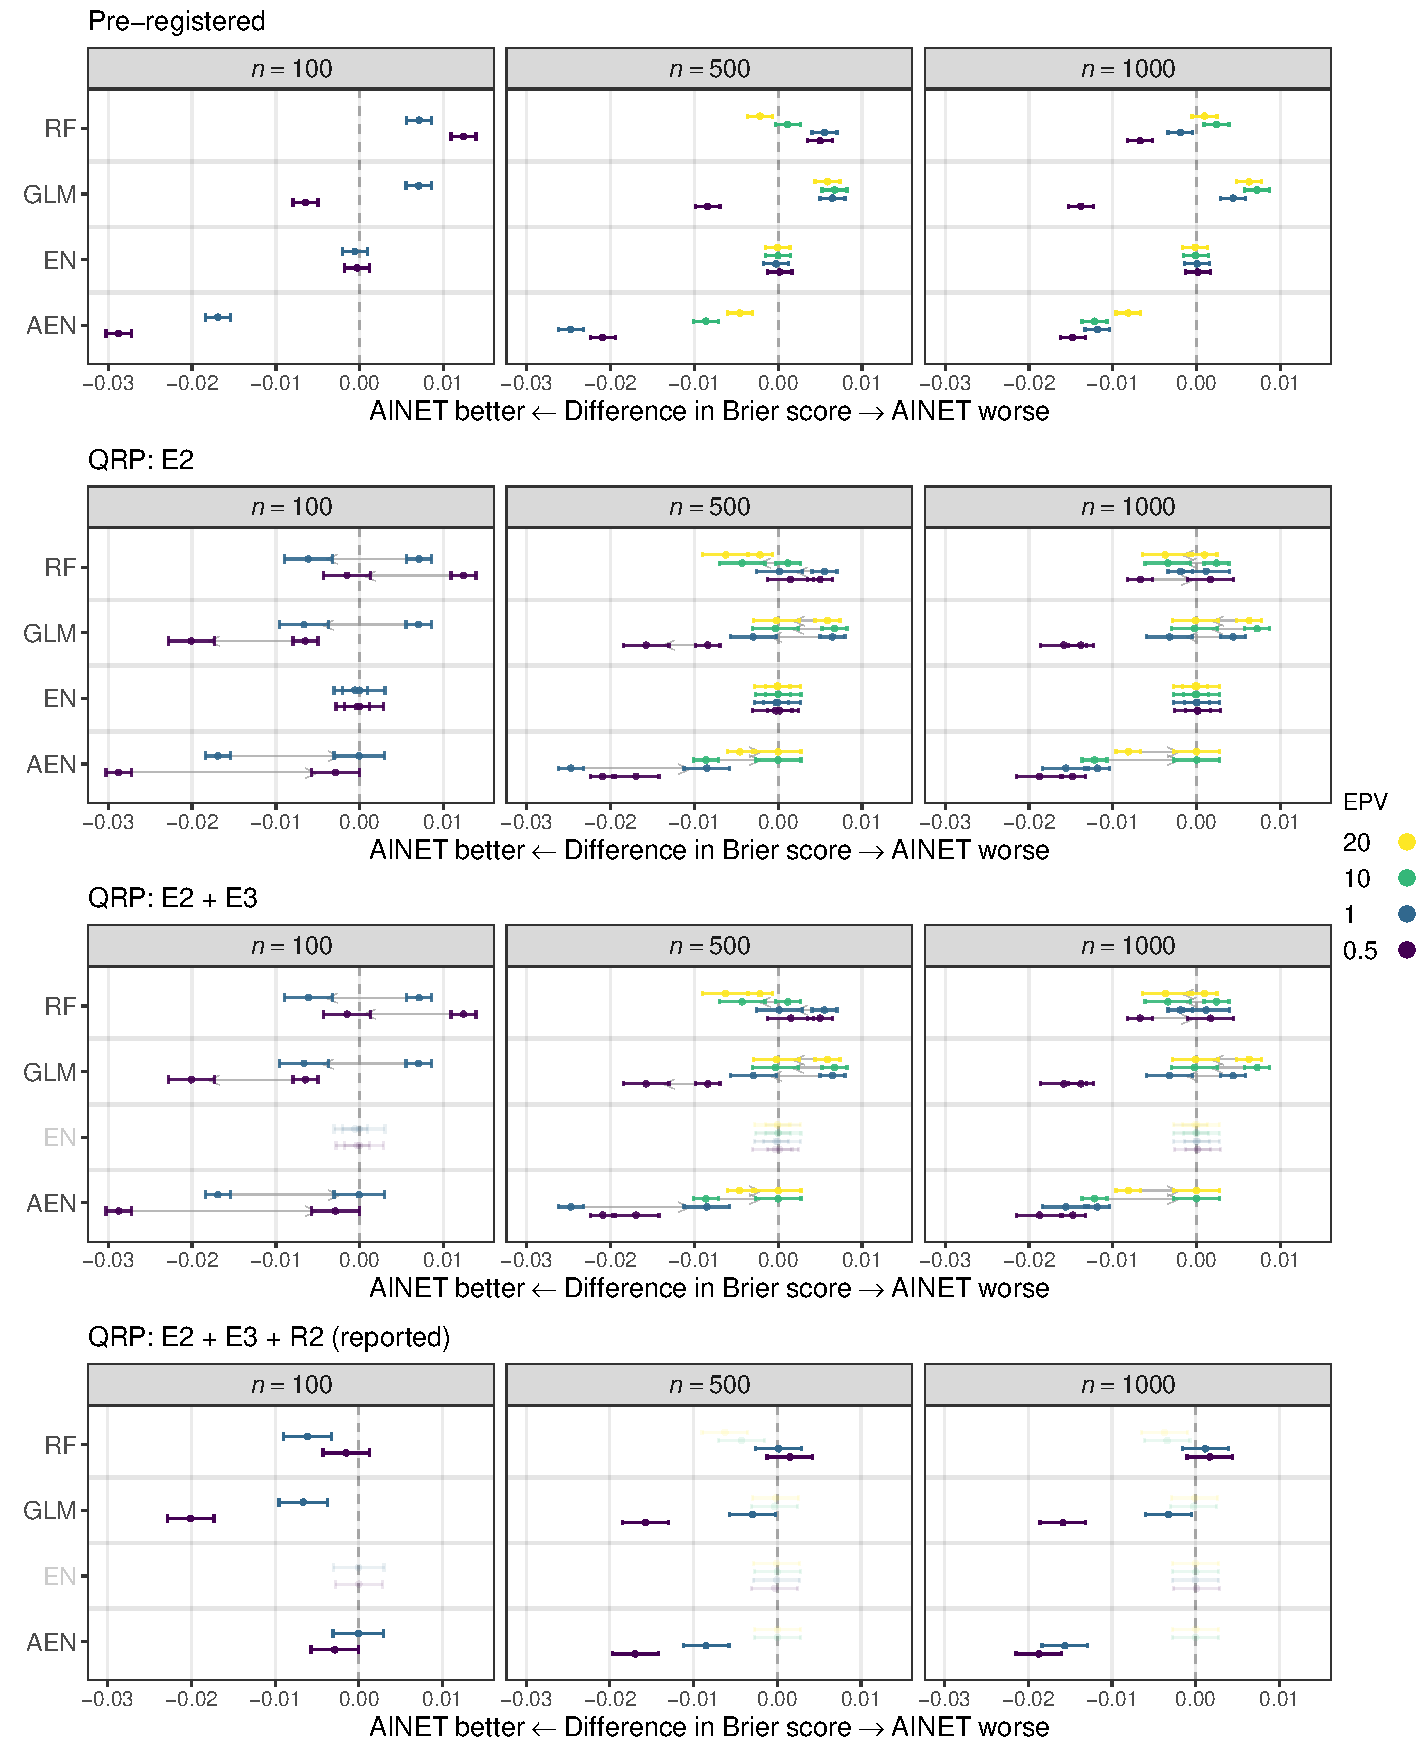
\includegraphics[width = 0.95\textwidth]{figure2.pdf}
  \caption{Differences in Brier score with 95\% adjusted confidence intervals
    between \ainet{} and random forest (RF),
    logistic regression (GLM), elastic net (EN) and adaptive elastic net (AEN)
    are shown for representative simulation conditions (correlated covariates
    $\rho = 0.95$, prevalence $\operatorname{prev} = 0.05$, a range of sample sizes
    $n$ and events per variable (EPV), in each simulation the Brier score is computed
    for 10'000 test observations; for details see Appendix~\ref{appendix:protocol}).
    The top row depicts the pre-registered results in which \ainet{} does not
    outperform any competitor uniformly, except AEN. In the second row, we apply
    QRP E2: Altering the data-generating process by adding a non-linear effect and
    sparsity. The gray arrows point from the pre-registered result to the results under
    the tweaked simulation. In the third row, QRP E3 is applied: EN is removed as
    a competitor. In the bottom row, selective reporting R2 is applied: Only low
    EPV settings are reported to give a more favorable impression for \ainet{}.
    Arrows are depicted only for non-overlapping confidence intervals.
    } \label{fig:E1}
\end{figure}
%--%--%--%--%--%--%--%--%--%--%--%--%--%--%--%--%--%--%--%--%--%--%--%--%--%--

We now show how application of QRPs changes the above pre-registered conclusions.
Figure~\ref{fig:E1} illustrates different types of QRPs sequentially applied
to simulation-based evaluation of \ainet{}. The top row depicts the
pre-registered differences in Brier score (horizontal axis) between \ainet{} and
competitor methods (vertical axis) for a representative subset of the simulation
conditions. A negative difference indicates superior performance of \ainet{}.
In the second row, the arrows depict the change in the pre-registered
results after changing the data-generating process (E2).
The third row shows the result after removal of the elastic net competitor
(E3). Finally, the bottom row shows the end result where selective reporting
of simulation conditions and competitor methods (R2) is applied to give
a more favorable impression of \ainet{}.
We will now discuss these QRPs in more detail.

\paragraph{Altering the data-generating process (E2)}
We could not detect a systematic performance benefit
of \ainet{} over standard logistic regression, elastic net regression, or
random forest for the scenarios specified in the protocol. For this reason,
we tweaked the data-generating process by adding different sparsity conditions and a
non-linear effect. We then found that
\ainet{} outperforms logistic regression under the following conditions:
Only few variables being associated with the
outcome (sparsity), a non-linear effect and a low number of events per
variable (EPV). Figure~\ref{fig:E1} (second row) shows the changes in Brier score
difference between the pre-registered and the tweaked simulation. As can be seen, the
tweaked data-generating process leads to \ainet{} being superior to competitors
in some conditions, and at least not inferior in others.

\paragraph{Removing competitor methods (E3)}
Despite the adapted data-generating process, we still observed only minor (if any)
improvements of \ainet{} over the elastic net. In order to present \ainet{}
in a better light we could omit the comparisons with the elastic net (E3),
as shown in Figure~\ref{fig:E1} (third row). This could be justified, for example,
by arguing that for neutral comparison it is sufficient to compare a less flexible
method (logistic regression, which has no tuning parameters and captures linear
effects), a more flexible method (random forest, which has tuning parameters and
captures nonlinear relationships), and a comparably flexible method (adaptive
elastic net, which has the same tuning parameters as AINET, but differs in the
way the penalization weights are chosen).

\paragraph{Selective reporting of simulation results (R2)}
After the removal of the competitor elastic net, there are still
some simulation conditions under which \ainet{} is not superior to
the remaining competitors. To make \ainet{} appear more favorable, we
thus report only simulation conditions with low EPV, as shown in
Figure~\ref{fig:E1} (fourth row).
This could be justified by the fact that journals require
authors to be concise in their reporting.
Otherwise, further conditions with low EPV values could be simulated to
make the results seem more exhaustive.
Focusing primarily on low EPV settings could be justified in
hindsight by framing \ainet{} as a method designed for high-dimensional
data (low sample size relative to the number of variables).

%%%%%%%%%%%%%%%%%%%%%%%%%%%%%%%%%%%%%%%%%%%%%%%%%%%%%%%%%%%%%%%%%%%%%%%%%%%%%%%%
\section{Recommendations}
\label{sec:recommendations}
%%%%%%%%%%%%%%%%%%%%%%%%%%%%%%%%%%%%%%%%%%%%%%%%%%%%%%%%%%%%%%%%%%%%%%%%%%%%%%%%

The previous sections painted a rather negative picture of how
undisclosed changes in simulation design, analysis and reporting
may lead to overoptimistic conclusions. In the
following, we summarize what we consider to be practical recommendations for
improving the methodological quality of simulation studies; see
Table~\ref{table:recommendations} for an overview. Our recommendations are
grouped with regards to which stakeholder they concern.

\begin{table}[!htb]
  \caption{Recommendations for improving quality of comparative simulation studies
    and preventing QRPs.}
  \label{table:recommendations}
  \centering
	\begin{tabular}{p{.95\textwidth}}
		\toprule
    \textit{Researchers} \\
    \midrule
    \vspace{-1.5em}
    \begin{itemize}
    \setlength\itemsep{0pt}
    \setlength\itemindent{-12pt}
        \item[--] Write (and possibly pre-register) simulation protocols
    \item[--] Adopt good computational practices (code review, packaging, unit-tests)
    \item[--] Share code and data (possibly in intermediate/summary form to enable
    secondary analysis)
    \item[--] Report the process of the simulation study fully and transparently
    (for instance, time-stamped protocol amendments to disclose pilot studies
    and \emph{post hoc} modifications)
    \item[--] Perform simulation analysis in a blinded manner
    \item[--] Collaborate with other research groups (possibly familiar with ``competing'' methods)
    \item[--] Disclose multiplicity and uncertainty of results (for example, with sensitivity analyses)
    \item[--] Teach simulation study methodology in statistics (post)graduate courses
    \end{itemize}

    \textit{Editors and reviewers} \\
    \midrule
    \vspace{-1.5em}
    \begin{itemize}
    \setlength\itemsep{0pt}
    \setlength\itemindent{-12pt}
    \item[--] Encourage exploration of conditions where methods should
    be inferior or break down
    \item[--] Encourage (pre-registered) simulation protocols
    \item[--] Provide enough space for description of simulation methodology
    \end{itemize}

    \textit{Journals and funding bodies} \\
    \midrule
    \vspace{-1.5em}
    \begin{itemize}
    \setlength\itemsep{0pt}
    \setlength\itemindent{-12pt}
    \item[--] Provide incentives for rigorous simulation methodology (such as badges on papers)
    \item[--] Require code and data
    \item[--] Promote standardized reporting
    \item[--] Adopt reproducibility checks
    \item[--] Promote/fund research and software to improve simulation study methodology
    \item[--] Shift focus away from outperforming state-of-the-art methods
    \end{itemize}\\
		\bottomrule
	\end{tabular}
\end{table}

\subsection{Recommendations for researchers}
Adopting pre-registered simulation protocols is an important measure
that researchers can take to prevent themselves from subconsciously engaging in QRPs.
Pre-registration enables readers to distinguish between confirmatory
and exploratory findings, and it lowers the risk of potentially flawed methods
being promoted as an improvement over competitors. While pre-registered
simulation protocols may at
first seem disadvantageous due to the additional work and possibly lower chance of publication,
they provide researchers with the means to differentiate their high-quality simulation
studies from the numerous unregistered and possibly less trustworthy simulation studies
in the literature.
Platforms such as GitHub (\url{https://github.com/}), OSF
(\url{https://osf.io/}), or Zenodo (\url{https://zenodo.org/}) can be used for
archiving and time-stamping documents. Moreover, pre-registration
can also save researchers from some work later on. For instance, large parts of the
methodology description can usually be copied from the protocol to the final manuscript.
% copy most parts of the simulation methodology description
% from the protocol to the final manuscript.

When pre-registering and conducting simulation studies, we recommend using a
robust computational workflow. Such a workflow encompasses packaging the software,
writing unit tests and reviewing code \citep[see][]{Schwab2021}.
Other researchers and the authors themselves then benefit from improved computational
reproducibility and less error-prone code.
Of course, there are also certain practical limits to computational
reproducibility. For instance, if a simulation study requires high performance
computing and/or several weeks of running time, the authors should not expect
reviewers and journals to replicate their simulation study from scratch. The authors
should nevertheless provide the code to run the simulation and, if possible, they should also provide
intermediate simulation results (for instance, fitted model objects) so that
the simulation study can at least be partially reproduced. Similarly,
authors can share the simulated data,
either in raw and/or some summarized form (for example, sharing simulated data
sets and parameter estimates of fitted models).
This allows interested readers and reviewers to do additional analyses.
Unlike experiments with human subjects, there are no privacy concerns for
sharing simulation data. Furthermore, online tools, such as INTEREST
\citep[INteractive Tool for Exploring REsults from Simulation
sTudies,][]{Gasparini2021}, can be used for interactive exploration of the data
set.

While planning a simulation study, it is impossible to think of all potential
weaknesses or problems that may arise when conducting the planned simulations.
In turn, researchers may be reluctant to tie their hands in a pre-registered protocol.
However, a transparently conducted and reported preliminary simulation can obviate most
of these problems. We recommend researchers to disclose preliminary results and any resulting
changes to the protocol, for example, in a revised and time-stamped version of the protocol.
This approach is similar to conducting a small pilot study, as is often done in non-simulation based
research. Even if researchers realize that further changes are required after the main simulation
study has begun, transparent reporting of when and why \emph{post hoc} modifications were made allows
the reader to better assess the quality of evidence provided by the study.
Researchers designing simulation studies may draw inspiration from clinical
trials by tracking their protocol modifications and time-stamping versions of their
protocol.

A different approach for making \emph{post hoc} changes to the protocol is to use
blinding in the analysis of the simulation results \citep{Dutilh2019}.
Blinded analysis is a standard procedure in particle physics to prevent
data analysts from biasing their result towards their own beliefs
\citep{Klein2005}, and it lends
legitimacy to \emph{post hoc} modifications of the simulation study.
For instance, researchers might shuffle the method labels and only unblind themselves
after the necessary analysis pipelines are set in place. An alternative blinding
approach is to carry out data generation and
analysis by different researchers.
For instance, the study from \citet{Kreutz2020} involved two independent research groups,
one who simulated and one who analyzed the data.
A related way for improving simulation studies is to collaborate with other
researchers, possibly ones familiar with ``competing'' methods. This helps to
design simulation studies which are more objective and whose results are more
useful for making a decision about which method to choose
under which circumstances.

We also recommend researchers to disclose the multiplicity and
uncertainty inherent to the design and analysis of their simulation studies
\citep{Hoffmann2021}. For instance, researchers can report sensitivity analyses
that show how the study results change for different analysis decisions
(for example, Table~4 in \citet{vanSmeden2016} shows how the evaluation
metrics for different estimators change depending on how convergence
of a method is defined). Methods from multivariate statistics can be used for
visualizing the influence of different design choices, such as the multidimensional
unfolding approach in \citet{Niessl2021}.

One reason for the low standards of simulation studies in the
statistics literature may be that rigorous simulation
methodology is usually not taught in graduate or postgraduate
courses (with a few exceptions, such as the course
``Using simulation studies to evaluate statistical methods''
from the MRC Clinical Trials Unit).
To improve training of current and future generations of statisticians, researchers who are
involved in teaching should therefore also include simulation
study methodology in their curricula.
The standards of simulation studies in many statistics
related fields (for instance, machine learning, psychometrics, econometrics,
or ecology) are arguably
not much different. One possible avenue for future research is
thus to also
promote education and adaptation of simulation study methodology
for the special needs in these fields.

\subsection{Recommendations for editors and reviewers}
Peer review is an important tool for identifying QRPs in research results
submitted to methodological journals.
For instance, reviewers may demand researchers to include competitor
methods which are not part of their comparison yet (or which might have been
excluded from the comparison). However, reviewers can only identify a subset
of all QRPs since some types are impossible to spot if no pre-registered
simulation protocol is in place (for example, a reviewer cannot know whether
the evaluation criterion was switched). Even QRPs which can be detected by peer
review may be difficult to spot in practice.
It is thus important that reviewers and editors promote that authors make
simulation protocols and computer code available alongside the manuscript.
Moreover, by providing enough space and encouraging authors to provide detailed
descriptions of their simulation studies, replicability of the simulation
studies can be improved. Finally, reviewers should not be satisfied with
manuscripts showing that a method is uniformly superior; they should
also encourage authors to explore conditions in which their method is
expected to be inferior to other methods or to break down entirely.

\subsection{Recommendations for journals and funding bodies}
Journals and funding bodies can improve on the status quo by either actively
requiring or passively incentivizing more rigorous and neutral simulation study
methodology. Actively, journals can make (pre-registered) simulation protocols
mandatory for all articles featuring a simulation study. A more passive and less
extreme measure would be to indicate with a badge whether an article contains
a pre-registered simulation study, or to introduce article types dedicated to
neutral comparison studies. Such an approach rewards researchers who take the
extra effort. Similar initiatives have led to a large increase in the adoption
of pre-registered study protocols in the field of psychology \citep{Kidwell2016}.
Another measure could be to require standardized reporting
of simulation studies, for example, the ``ADEMP'' reporting structure proposed by
\citet{Morris2019}. Journals may also employ reproducibility checks to ensure
computational reproducibility of the published simulation studies. This is
already done, for example, by the Journal of Open Source Software or the Journal
of Statistical Software. Moreover, journals and funding bodies can promote or fund
research and software to improve simulation study methodology. For instance, a
journal might have special calls for papers on simulation methodology. Similarly,
a funding body could have special grants dedicated to software development
that facilitates sound design, execution and reporting of simulation studies
\citep[as][]{White2010, Gasparini2018, Chalmers2020}.
Finally, journals and funding bodies often exert a strong incentive on researchers
to publish novel and superior methods. This may lead to articles with
non-systematic simulation studies that mainly highlight settings beneficial
to the proposed methods. We believe that the above recommendations
can shift the incentive structure towards more transparent and neutral
simulation studies, and away from the ``one method fits all data sets''
philosophy \citep{Strobl2022}.

%%%%%%%%%%%%%%%%%%%%%%%%%%%%%%%%%%%%%%%%%%%%%%%%%%%%%%%%%%%%%%%%%%%%%%%%%%%%%%%%
\section{Conclusions} \label{sec:discussion}
%%%%%%%%%%%%%%%%%%%%%%%%%%%%%%%%%%%%%%%%%%%%%%%%%%%%%%%%%%%%%%%%%%%%%%%%%%%%%%%%

Simulation studies should be viewed and treated analogously to (empirical)
experiments from other fields of science. Transparent reporting of methodology
and results is essential to contextualize the outcome of such a study. As in
other empirical sciences, QRPs in simulation studies can obfuscate the usefulness
of a novel method and lead to misleading and non-replicable results.

By deliberately using several QRPs we were able to present a method with no expected
benefits and little theoretical justification -- invented solely for this article -- as an
improvement over theoretically and empirically well-established competitors.
While such intentional engagement in these practices is far from the norm,
unintentional QRPs may have the same detrimental effect.
We hope that our illustration will increase awareness about the fragility of
findings from simulation studies and the need for higher standards.

While this article focuses on comparative simulation studies, many of the issues
and recommendations also apply to neutral comparison studies with real data sets
as discussed in \citet{Niessl2021}. Some of the noted problems even exist in
theoretical research; due to the incentive to publish positive results, researchers
often selectively study optimality conditions of methods rather than conditions
under which they fail.

Again, it is imperative to note that researchers rarely engage in QRPs with malicious
intent but because humans tend to interpret ambiguous information self-servingly, and
because they are good at finding reasonable justifications that match their expectations
and desires \citep{Simmons2011}. As in other domains of science, it is easier to publish
positive results in methodological research, that is, novel and superior methods
\citep{Boulesteix2015}. Thus, methodological researchers will typically desire to show
the superiority of a method rather than to neutrally disclose its strengths and
weaknesses.

We provide several recommendations involving various stakeholders in the research
community which we believe may help incentivize researchers to perform well-designed
simulation studies.
Most importantly, we think that reviewers, journals and funders should raise
the standards for simulation studies by promoting pre-registered simulation protocols
and rewarding researchers who invest the extra effort. Although there is evidence for
the effectiveness of protocols in preventing QRPs in other fields, it is unclear
whether this effect translates to simulation studies. Indeed, there are many reasons
to believe that simulation studies will not benefit in a similar way as studies with
human or animal subjects, due to the nature of simulations studies. For instance,
requiring pre-registered protocols cannot prevent researchers engaging in QRPs until
they find their desired results and only then writing and registering a protocol.
In addition, there is currently no tradition of pre-registration in simulation studies,
no best-practices guidance and no dedicated platform to publish protocols. For example,
\citet{Kipruto2022} published the pre-registration of their simulation protocol as a
journal article, whereas the pre-registration of the protocol from our study was uploaded
to GitHub. Both protocols use the ADEMP reporting structure from \citet{Morris2019}, yet
the field could benefit from reporting guidelines
developed by a consortium of simulation experts
similar to the guidelines for health research promoted by the
EQUATOR Network \citep{Altman2008}. Similarly, the field could benefit from a centralized
pre-registration platform tailored to simulation studies (similar to
\url{https://clinicaltrials.gov} for clinical trials).
Regardless of the (unknown) effectiveness of pre-registered simulation protocols,
we personally think that they are an important step toward improving simulation studies
since they promote a minimum degree of transparency and credibility. For this reason, we think
that they are especially important for ``late-stage'' methodological studies
\citep{Heinze2022} where the objective is to neutrally compare different methods and
generate robust evidence.

\section*{Software and data}
The simulation study was conducted in the \textsf{R} language for statistical
computing \citep{pkg:base} using the version 4.1.1. The method
\ainet{} is implemented in the \pkg{ainet} package and available on GitHub
(\url{https://github.com/LucasKook/ainet}). We provide scripts for
reproducing the different simulation studies on the GitHub repository
(\url{https://github.com/SamCH93/SimPaper}).
Due to the computational overhead, we also provide the resulting data
so that the analyses can be conducted without rerunning the simulations.
We used \pkg{pROC} version 1.18.0 to compute the AUC \citep{pkg:proc}.
Random forests were fitted using \pkg{ranger} version 0.13.1 \citep{ranger2017}.
For penalized likelihood methods, we used \pkg{glmnet} version 4.1.2
\citep{Friedman2010,Simon2011}.
The \pkg{SimDesign} package version 2.7.1 was used to set up simulation scenarios
\citep{Chalmers2020}.

\section*{Acknowledgements}
We thank Eva Furrer, Malgorzata Roos and Torsten Hothorn for
helpful discussion and comments on the simulation protocol and drafts of the
manuscript.
We also thank the anonymous referees and the associate editor for constructive
and valuable comments that improved the manuscript substantially.
Our acknowledgement of these individuals does not imply their endorsement of this article.
The authors declare that they do not have any conflicts of interest.
SP acknowledges financial support from the Swiss National Science Foundation
(Project~\#189295). The funder had no role in study design, data collection,
data analysis, data interpretation, decision to publish, or preparation of
the manuscript.

% Appendix
% ======================================================================
\begin{appendices}

\section{Simulation protocol}
\label{appendix:protocol}

Below, we include an excerpt of the final version of the protocol for the
simulation-based evaluation of \ainet{}. All time-stamped versions
of the protocol are available at \url{https://doi.org/10.5281/zenodo.6364575}.

%%%%%%%%%%%%%%%%%%%%%%%%%%%%%%%%%%%%%%%%%%%%%%%%%%%%%%%%%%%%%%%%%%%%%%%%%%%%%%%%
\subsection{Aims} \label{sec:aims}
%%%%%%%%%%%%%%%%%%%%%%%%%%%%%%%%%%%%%%%%%%%%%%%%%%%%%%%%%%%%%%%%%%%%%%%%%%%%%%%%

The aim of this simulation study is to systematically study the predictive
performance of \ainet{} for a binary prediction task. The simulation conditions
should resemble typical conditions found in the development of prediction models
in biomedical research. In particular we want to evaluate the performance of
\ainet{} conditional on
\begin{itemize}
  \item low- and high-dimensional covariates
  \item (un-)correlated covariates
  \item small and large sample sizes
  \item varying baseline prevalences
\end{itemize}
\ainet{} will be compared to other (penalized) binary regression models
from the literature, namely
\begin{itemize}
  \item Binary logistic regression: the simplest and most popular method for
        binary prediction
  \item Elastic net: a generalization of LASSO and ridge regression, the most
        widely used penalized regression methods
  \item Adaptive elastic net: a generalization of the most popular weighted 
  penalized regression method (adaptive LASSO)
  \item Random forest: a popular, more flexible method. This method is related to
        \ainet{}, see Section~\ref{sec:methods}.
\end{itemize}
These cover a wide range of established methods with varying flexibility and
serve as a reasonable benchmark for \ainet. There are many more extensions of
the adaptive elastic net in the literature \citep[see \eg{} the review
by][]{Vidaurre2013}. However, most of these extensions focus on variable
selection and estimation instead of prediction, which is why we restrict our
focus only on the four methods above.

%%%%%%%%%%%%%%%%%%%%%%%%%%%%%%%%%%%%%%%%%%%%%%%%%%%%%%%%%%%%%%%%%%%%%%%%%%%%%%%%
\subsection{Data-generating process} \label{sec:dgp}
%%%%%%%%%%%%%%%%%%%%%%%%%%%%%%%%%%%%%%%%%%%%%%%%%%%%%%%%%%%%%%%%%%%%%%%%%%%%%%%%

In each simulation $b = 1, \dots, B$, we generate a data set consisting of $n$
realizations, \ie $\{(\ry_i, \rx_i)\}_{i=1}^n$. A datum $(\rY, \rX)$ consists of
a binary outcome $\rY \in \{0, 1\}$ and $p$-dimensional covariate vector
$\rX \in \RR^p$. The binary outcomes are generated by
\begin{align*}
  Y \given \rx &\sim \BD\left(\expit\left\{\beta_0 +
	\rx^\top\shiftparm\right\}\right)
\end{align*}
with $\expit(z) = (1 + \exp(-z))^{-1}$ and the covariate vectors are generated by
\begin{align*}
  \rX &\sim \ND_p\left(0, \Sigma\right)
\end{align*}
with covariance matrix $\Sigma$ that may vary across simulation conditions (see
below). The baseline prevalence is $\prev = \expit(\beta_0)$. The coefficient
vector $\shiftparm$ is generated from
\begin{align*}
  \shiftparm \sim \ND_p(0, \Id)
\end{align*}
once per simulation. Finally, the simulation parameters are varied fully
factorially (except for the removal of some unreasonable conditions) as
described below, leading to a total of 128 scenarios.

\subsection*{Sample size}
The sample size used in the development of predictions models varies widely
\citep{Damen2016}. We will use $n \in \{100, 500, 1000, 5000\}$, which span
typical values occurring in practice. Note that previous simulation studies
usually chose sample size based on the implied number of events together with
the number of covariates in the model for easier interpretation
\citep{vanSmeden2018, Riley2018}. We will use this approach in reverse to
determine the dimensionality of the parameters below.

\subsection*{Dimensionality}
Previous simulation studies showed that events per variable ($\EPV$) rather than
the absolute sample size $n$ and dimensionality $p$ influences the predictive
performance of a method. We will therefore define the dimensionality $p$ via EPV
by $$p = \frac{n \cdot \prev}{\EPV}$$ and $2 \leq p \leq 100.$ If the above
formula gives non-integer values, the next larger integer will be used for $p$.
When the formula gives values above 100 or below 2, this simulation condition
will be removed from the design. This is done because prediction models are in
practice only multivariable models ($p \geq 2$), but at the same time the number
of predictors is rarely larger than $p \geq 100$
\citep{Kreuzberger2020,Seker2020, Wynants2020}. The exception are studies
considering complex data, such as images, omics, or text data which are not the
focus here. The values $\EPV \in \{20, 10, 1, 0.5\}$ are chosen to cover
scenarios with small to large number of covariates \citep[see][]{vanSmeden2018}.

\subsection*{Collinearity in $\rX$}
We distinguish between no, low, medium and high collinearity. The diagonal
elements of $\Sigma$ are given by $\Sigma_{ii} = 1$ and the off-diagonal
elements are set to $\Sigma_{ij} = \rho$, $\rho \in \{0, 0.3, 0.6, 0.95\}$.
These values cover the typical (positive) range of correlations.

\subsection*{Baseline prevalence}
Different baseline prevalences $\expit(\beta_0) \in \{0.01, 0.05, 0.1\}$ are 
considered, reflecting a reasonable range of prevalences for rare to
common diseases/adverse events.

\subsection*{Test data}
In order to test the out-of-sample predictive performance, we generate a test
data set of $n_{\text{test}} = 10000$ data points in each simulation $b$.

%%%%%%%%%%%%%%%%%%%%%%%%%%%%%%%%%%%%%%%%%%%%%%%%%%%%%%%%%%%%%%%%%%%%%%%%%%%%%%%%
\subsection{Estimands} \label{sec:estimands}
%%%%%%%%%%%%%%%%%%%%%%%%%%%%%%%%%%%%%%%%%%%%%%%%%%%%%%%%%%%%%%%%%%%%%%%%%%%%%%%%
We will estimate different quantities to evaluate overall predictive
performance, calibration, and discrimination, respectively. All methods will be
evaluated on independently generated test data.

\subsubsection{Primary estimand}

\begin{itemize}
  \item \textbf{Brier score.} We compute the Brier score as
  $$\BS = n_{\text{test}}^{-1} \sum_{i=1}^{n_{\text{test}}} (y_{i} - \hat{y}_{i})^2,$$
        where $\hat{y} = \widehat\Prob(Y = 1 \given \rx)$. Lower values indicate
        better predictive performance in terms of calibration and sharpness. A
        prediction is well-calibrated if the observed proportion of events is
        close to the predicted probabilities. Sharpness refers to how
        concentrated a predictive distribution is (\eg{} how wide/narrow a
        prediction interval is), and the predictive goal is to maximize
        sharpness subject to calibration \citep{Gneiting2008}. The Brier score
        is a proper scoring rule, meaning that it is minimized if a predicted
        distribution is equal to the data-generating distribution
        \citep{Gneiting2007}. Proper scoring rules thus encourage honest
        predictions. The Brier score is therefore a principled choice for our
        primary estimand.
\end{itemize}

\subsubsection{Secondary estimands}
\begin{itemize}
  \item \textbf{Scaled Brier score.} The scaled Brier score (also known as Brier
        skill score) is computed as
  $$\BS^{*} = 1 - \BS/\BS_{0}$$
        with $\BS_{0} = \bar{y}(1 - \bar{y})$ and $\bar{y}$ the observed
        prevalence in the data set. The scaled Brier score takes into account
        that the prevalence varies across simulation conditions. Hence, the
        scaled Brier score can be compared between conditions \citep{Schmid2005,
        steyerberg2019clinical}.

  \item \textbf{Log-score.} We compute the log-score on independently generated test data,
  $$\LS = - n_{\text{test}}^{-1} \sum_{i=1}^{n_{\text{test}}} \left\{ y_{i} \log(\hat{y}_{i})
        + (1 - y_{i}) \log (1 - \hat{y}_{i})\right\},$$ will be used as a
        secondary measure of overall predictive performance. Lower values
        indicate better predictive performance in terms of calibration and
        sharpness. The log-score is a strictly proper scoring rule, however, it
        is more sensitive to extreme predicted probabilities compared to the
        Brier score \citep{Gneiting2007}.
  
  \item \textbf{AUC.} The AUC is the area under the
        receiver-operating-characteristic (ROC) curve
        \citep{steyerberg2019clinical}. It will be used as a measure of
        discrimination and values closer to one indicate better discriminative
        ability. Discrimination describes the ability of a prediction model to
        discriminate between cases and non-cases. Other discrimination measures,
        such as accuracy, sensitivity, specificity, etc., are not considered
        because we want to evaluate predictive performance in terms of
        probabilistic predictions instead of point predictions/classification.

  \item \textbf{Calibration slope $\hat b$.} The calibration slope $\hat b$ is
        obtained by regressing the test data outcomes $y_{\text{test}}$ on the
        models' predicted logits $\logit({\hat{y}})$, \ie
  $$\logit\Ex[Y \given \hat\ry] = a + b\logit(\hat\ry).$$
        This measure will be used to assess calibration and deviations of
        $\hat b$ from one indicate miscalibration
        \citep{steyerberg2019clinical}.

  \item \textbf{Calibration in the large $\hat a$.} We inspect calibration in
        the large $\hat a$ on independently generated test data, from the model
  $$\logit\Ex[Y \given \hat\ry] = a + \logit(\hat{y}).$$
        This measure will also be used to assess calibration and deviations of
        $\hat a$ from zero indicate miscalibration
        \citep{steyerberg2019clinical}.
\end{itemize}

To facilitate comparison between simulation conditions, all estimands will also
be corrected by the oracle version of the estimand, \eg{} the Brier score will
be computed from the ground truth parameters and the simulated data $\rx$,
subsequently the oracle Brier score will be subtracted from the estimated Brier
score.

%%%%%%%%%%%%%%%%%%%%%%%%%%%%%%%%%%%%%%%%%%%%%%%%%%%%%%%%%%%%%%%%%%%%%%%%%%%%%%%%
\subsection{Methods} \label{sec:methods}
%%%%%%%%%%%%%%%%%%%%%%%%%%%%%%%%%%%%%%%%%%%%%%%%%%%%%%%%%%%%%%%%%%%%%%%%%%%%%%%%

\subsubsection{\ainet}
We now present the mock-method and give a superficial motivation why it could
lead to improved predictive performance: Choosing the vector of penalization
weights in the adaptive LASSO becomes difficult in high-dimensional settings.
For instance, using absolute LASSO estimates as penalization weights omits the
importance of several predictors by not selecting them, especially in the case
of highly correlated predictors \citep{Algamal2015}. The adaptive importance
elastic net (\ainet{}) circumvents this problem by employing a random forest to
estimate the penalization weights via an \emph{a priori} chosen variable
importance measure. In this way, the importance of all variables enter the
penalization weights simultaneously.

The penalized log-likelihood for \ainet{} for a single observation $(\ry, \rx)$
is defined as
$$\ell_{\text{AINET}}(\beta_0, \shiftparm; \ry, \rx, \alpha, \lambda, \wvec) = 
  \ell(\beta_0, \shiftparm; \ry, \rx) + \aipen$$
where
$$\ell(\beta_0, \shiftparm; \ry, \rx) = 
\ry \log\left(\expit\left\{\beta_0 + \linpred\right\}\right) + (1 - \ry) \log\left(1 - \expit\left\{\beta_0 + \linpred\right\}\right)$$
denotes the log-likelihood of a binomial GLM and $\wvec$ is derived from a
random forest variable importance measure $\widetilde\IMP$ as
$$w_j = 1 - \left(\frac{\IMP_j}{\sum_{k=1}^p \IMP_k}\right)^\gamma,$$
where we transform $\IMP$ to be non-negative via
% $$\IMP = \widetilde\IMP - \min_j\{\widetilde{\IMP}_j\},$$
% or
$$\IMP_j = \max\{0, \widetilde\IMP_j\}$$
and $\gamma$ is a hyperparameter for the influence of the weights similar to
$\gamma$ hyperparameter of the adaptive elastic net. \ainet{} is fitted by
maximizing its penalized log-likelihood assuming i.i.d. observations
$\{(\ry_i, \rx_i)\}_{i=1}^n$, \ie
$$\arg\max_{\beta_0, \shiftparm} \sum_{i = 1}^n \ell_{\text{AINET}}(\beta_0,
\shiftparm; \ry_i, \rx_i, \alpha, \lambda, \wvec).$$

Per default, we choose mean decrease in the Gini coefficient for
$\widetilde\IMP$. Hyperparameters of the random forest are not tuned, but kept
at their default values (\eg{} \code{mtry}, \code{ntree}). The hyperparameter
$\gamma = 1$ will stay constant for all simulations.

\ainet{} is supposed to seem like a reasonable method at first glance. However,
\ainet{} cannot be expected to share desirable theoretical properties with the
usual adaptive LASSO, such as oracle estimation \citep{Zou2006}. This is because
the penalization weights $\wvec$ do not meet the required consistency
assumption. Also in terms of prediction performance, \ainet{} is not expected to
outperform methods of comparable complexity.

\subsubsection{Benchmark methods}

\begin{itemize}
  \item \textbf{Binary logistic regression} \citep{mccullagh2019generalized}
        with and without ridge penalty for high- and low-dimensional settings,
        respectively. In case a ridge penalty is needed, it is tuned via 5-fold
        cross-validation by following the ``one standard error'' rule as
        implemented in \pkg{glmnet} \citep{Friedman2010}.
  \item \textbf{Elastic net} \citep{Zou2005}, for which the penalized
        log-likelihood is given by
    $$\ell_{\text{EN}}(\beta_0, \shiftparm; \ry, \rx, \alpha, \lambda) = 
        \ell(\beta_0, \shiftparm; \ry, \rx) + \llpen.$$ Here, $\alpha$ and
        $\lambda$ are tuned via 5-fold cross-validation by following the ``one
        standard error'' rule.
  \item \textbf{Adaptive elastic net} \citep{Zou2006}, with penalized loss
        function
    $$\ell_{\text{adaptive}}(\beta_0, \shiftparm; \ry, \rx, \alpha, \lambda, \wvec)
        = \ell(\beta_0, \shiftparm; \ry, \rx) + \aipen.$$ Here, the penalty
        weights $\wvec$ are inverse coefficient estimates from a binary logistic
        regression
    $$\hat{w}_j = \lvert\hat\eparm_j\rvert^{-\gamma},$$
        where $\lambda$ and $\alpha$ are tuned via 5-fold cross-validation by
        following the ``one standard error'' rule. The hyperparameter
        $\gamma = 1$ will stay constant for all simulations. In case $p > n$, we
        estimate the penalty weights using a ridge penalty, tuned via an
        additional nested 5-fold cross-validation by following the ``one
        standard error'' rule.
  \item \textbf{Random forests} \citep{Breiman2001} for binary outcomes without
        hyperparameter tuning. The default parameters of \pkg{ranger} will be
        used \citep{ranger2017}. % , \ie
    % \code{ntree = 500}, \code{mtry = floor(sqrt(p))}, \code{min.node.size = },
    % \code{max.depth = }, \code{sample.fraction = }
\end{itemize}


%%%%%%%%%%%%%%%%%%%%%%%%%%%%%%%%%%%%%%%%%%%%%%%%%%%%%%%%%%%%%%%%%%%%%%%%%%%%%%%%
\subsection{Performance measures} \label{sec:performance}
%%%%%%%%%%%%%%%%%%%%%%%%%%%%%%%%%%%%%%%%%%%%%%%%%%%%%%%%%%%%%%%%%%%%%%%%%%%%%%%%

The distribution of all estimands from Section~\ref{sec:estimands} will be
assessed visually with box- and violin-plots that are stratified by method and
simulation conditions. We will also compute mean, median, standard deviation,
interquartile range, and 95\% confidence intervals for each of the estimands.
Moreover, instead of ``eye-balling'' differences in predictive performance
across methods and conditions, we will formally assess them by regressing the
estimands on the method and simulation conditions \citep[\cf][]{Skrondal2000}.
To do so, we will use a fully interacted model with the interaction between the
methods and the 128 simulations conditions, \ie in R notation: \texttt{estimand
  $\sim$ 0 + method:scenario}. We will rank pairwise comparison between two
methods within a single condition by their $p$-values, to more easily identify
conditions where methods show differences in predictive performance. The choice
of a significance level at which a method is deemed superior will be determined
based on preliminary simulations. We set this level to 5\%, where $p$-values
will be adjusted using the single-step method \citep{pkg:multcomp} within a
single simulation condition for comparisons between \ainet{} and any other
method.


\subsection{Determining the number of simulations}

We determine the number of simulation $B$ such that the Monte Carlo standard
error of the primary estimand, the mean Brier score $\BS/B$, is sufficiently
small. The variance of $\BS/B$ is given by
\begin{align*}
  \Var\left(\BS/B\right)
  &= \frac{\Var\left\{(y -
    \hat{y})^{2}\right\}}{B \cdot n_{\text{test}}}
  % &= B^{-1}n_{\text{test}}^{-1} \left\{\Ex[(y_{ib} - \hat{y}_{ib})^{4}] -
  %   \Ex[(y_{ib} - \hat{y}_{ib})^{2}]^{2}\right\}
\end{align*}
and $\Var\left\{(y_{ib} - \hat{y}_{ib})^{2}\right\}$ could be decomposed further
\citep{Bradley2008}. However, the resulting expression is difficult to evaluate
for our data-generating process as it depends on several of the simulation
parameters. We therefore follow a similar approach as in \citet{Morris2019} and
estimate $\widehat{\Var}\left\{(y_{ib} - \hat{y}_{ib})^{2}\right\} < V$ from an
initial small simulation run with 100 simulations per condtion to get an upper
bound $V$ for worst-case variance across all simulation conditions. Therefore,
the number of simulations is then given by
$$B = \frac{V}{n_{\text{test}} \Var\left(\BS\right)}.$$
Since $\BS \in [0, 1]$ we decide that we require the Monte Carlo standard error
of $\BS$ to be lower than four significant digits, $0.0001$.

The initial simulation run led to an estimated worst case variance of
$\widehat{V} = 0.2$. Therefore, we compute that
$$B = 0.2/(10000 \times 0.0001^{2}) = 2000$$
replications are required to obtain Brier score estimates with the
desired precision.

%%%%%%%%%%%%%%%%%%%%%%%%%%%%%%%%%%%%%%%%%%%%%%%%%%%%%%%%%%%%%%%%%%%%%%%%%%%%%%%%
\subsection{Handling exceptions} \label{sec:exceptions}
%%%%%%%%%%%%%%%%%%%%%%%%%%%%%%%%%%%%%%%%%%%%%%%%%%%%%%%%%%%%%%%%%%%%%%%%%%%%%%%%
It is inevitable that convergence issues and other problems will arise in the
simulation study. We will handle them as follows:
\begin{itemize}
  \item If a method fails to converge, the simulation will be excluded from the
        analysis. The failing simulations will not be replaced with new
        simulations that successfully converge as convergence may be impossible
        for some scenarios.
  \item We will report the proportion of simulations with convergence issues for
        each method and discuss the potential reasons for their emergence.
  \item In case of severe convergence issues or other problems (more than 10\%
        of the simulations failing within a setting), we may adjust the
        simulation parameters post hoc. This will be indicated in the discussion
        of the results.
  \item Convergence may be possible for certain tuning parameters of a method
        (\eg{} cross-validation of LASSO may fail for some values $\lambda$
        while it could work for others). In this case we will choose a parameter
        value where the method still converges, as one would usually do with a
        real data set.
\end{itemize}


% \section{Pre-registered results}
% \label{appendix:pre-registered-results}
% 
Here, we describe the outcomes of the preregistered simulations.
Overall, the performance of \ainet{} was virtually identical to elastic net
regression. The adaptive penalization weights of \ainet{} do not seem to make a
difference for the data generating mechanism considered in our simulations.
Moreover, since the data were generated under a process equivalent to a logistic
regression model, it is no surprise that for reasonably large sample sizes,
logistic regression also performed the best. The only exception are
conditions with small sample size and low number of events per variable. Here,
\ainet{} and elastic net led to more stable and better calibrated predictions
than logistic regression. The random forest was outperformed by \ainet{} in most
simulation conditions, with exception of very small sample size and prevalence,
as well as when a high correlation between covariates was present. Finally, the
performance of the adaptive elastic net was generally worse compared to
\ainet{} and elastic net. In the following, we summarize the results for each
estimand.

%%%%%%%%%%%%%%%%%%%%%%%%%%%%%%%%%%%%%%%%
\subsection{Brier score (primary estimand)}
%%%%%%%%%%%%%%%%%%%%%%%%%%%%%%%%%%%%%%%%
Figure~\ref{fig:tiebrier} shows the differences in mean Brier score between
\ainet{} and the other methods stratified by simulation conditions.
% elastic net
We see that there is hardly any difference between \ainet{} and the elastic net (EN)
across all simulation conditions meaning that predictive performance of both
methods seems to be very similar in the investigated scenarios.

% random forest
The random forest (RF) shows better predictive performance than \ainet{} in
conditions with very low sample size ($n = 100$) and prevalence
($\mbox{prev} = 0.01$). For increasing sample size and prevalence, the
performance of \ainet{} seems to become more similar or improve over RF when the
correlation of the covariates is not too large ($\rho \leq 0.6$) especially for
low events per variable ($\mbox{EPV} \leq 1$). For highly correlated covariates
($\rho = 0.95$), the performance of \ainet{} is similar or worse across most
simulation conditions.

% GLM
Logistic regression (GLM) showed better predictive performance compared to
\ainet{} in most simulation conditions. An exception are the conditions with
small sample size ($n = 100$), medium to large prevalence
($\mbox{prev} \geq 0.05$) and low events per variable ($\mbox{EPV} \leq 1$),
where \ainet{} performed better than GLM.

The adaptive elastic net (AEN) method performed worse than \ainet{} in almost
all simulation conditions. Only in conditions with very large sample size
($n = 5000$), very small prevalence ($\mbox{prev} = 0.01$), and high events per
variable ($\mbox{EPV} = 20$), AEN showed predictive performance on par with
\ainet{}.

%%%%%%%%%%%%%%%%%%%%%%%%%%%%%%%%%%%%%%%%
\subsection{Scaled Brier score (secondary estimand)}
%%%%%%%%%%%%%%%%%%%%%%%%%%%%%%%%%%%%%%%%
Figure~\ref{fig:tiesbrier} shows the differences in scaled Brier score between
\ainet{} and the other methods stratified by simulation conditions. The scaled
Brier score is useful to compare the actual values of Brier scores across
conditions with different prevalence, but not so much to compare Brier scores of
different methods within a simulation condition with fixed prevalence.

We see that for most conditions the plots look like a flipped version of the
original Brier scores from Figure~\ref{fig:tiebrier}. Therefore, conclusions are
mostly the same. For very small sample sizes coupled with low prevalence and low
events per variable (the topleft plots), the scaled Brier score indicates
superiority of \ainet{} over RF and GLM, which is opposite the conclusion based
on the raw Brier score. We advise to interpret these conditions cautiously since
the prevalence prediction which is used for scaling is based on the much larger
test data set.

%%%%%%%%%%%%%%%%%%%%%%%%%%%%%%%%%%%%%%%%
\subsection{Log-score (secondary estimand)}
%%%%%%%%%%%%%%%%%%%%%%%%%%%%%%%%%%%%%%%%
Figure~\ref{fig:tienll} shows the differences in log-score between \ainet{} and
the other methods stratified by simulation conditions. We see that in certain
conditions, the error bars of certain methods are much larger. This is due to
the log-score's sensitivity to extreme predictions, which often happen under the
RF (and sometimes under the GLM). Despite the larger variability of the log-score,
conclusion regarding the comparison between \ainet{} and the other
methods are largely the same as under the Brier score.

%%%%%%%%%%%%%%%%%%%%%%%%%%%%%%%%%%%%%%%%
\subsection{Area under the curve (secondary estimand)}
%%%%%%%%%%%%%%%%%%%%%%%%%%%%%%%%%%%%%%%%
Figure~\ref{fig:tienll} shows the differences in area under the curve (AUC)
between \ainet{} and the other methods stratified by simulation conditions.
As with the other estimands, \ainet{} shows virtually identical performance
as EN regression across all simulation conditions.
\ainet{} seems to outperform RF across most simulation conditions, with the
exception of a conditions with low sample size ($n = 100$), medium prevalence
($\mbox{prev} = 0.05$), and low events per variable ($\mbox{EPV} \leq 1$).
GLM, typically outperforms \ainet{} conditions with small to medium sample size
($n \leq 500$), and also in conditions with larger sample size when the
events per variable is normal to high ($\mbox{EPV} \geq 10$) and the prevalence
is small ($\mbox{prev}  = 0.01$).
Finally, the AEN is worse with respect to AUC than \ainet{} across all
simulation conditions.

%%%%%%%%%%%%%%%%%%%%%%%%%%%%%%%%%%%%%%%%
\subsection{Calibration slope (secondary estimand)}
%%%%%%%%%%%%%%%%%%%%%%%%%%%%%%%%%%%%%%%%
Figure~\ref{fig:cslope} shows boxplots of calibration slopes stratified by
simulation condition and method. For each condition the percentage of
simulations where no estimate could be obtained is indicated. This usually
happened because of extreme (close to zero or one) predictions, or
non-convergence of the method itself. We caution against interpretation of the
random forest (RF) calibration slopes because this method often resulted in
predicted probabilities of zero or one, so that a calibration slope could not
be fitted.

We see that logistic regression (GLM) shows on average optimal calibration slopes
in most simulation condition. In cases where it is off one, its calibration
slopes are usually too small indicating overoptimistic predictions. In general,
worse calibration slopes are obtained for lower event per variable (EPV).

The penalized methods (\ainet{}, EN, AEN) show a more stable behavior, and on
average larger calibration slopes than GLM. This is likely confounded by the
simulation conditions in which no GLM calibration slope can be estimated, but
estimation of the penalized methods' calibration slope is still possible. Among
the penalized method's \ainet{} and EN shows relatively similar calibration
slopes whereas the AEN shows worse calibration slopes that are more off the
value of one.

%%%%%%%%%%%%%%%%%%%%%%%%%%%%%%%%%%%%%%%%
\subsection{Calibration in the large (secondary estimand)}
%%%%%%%%%%%%%%%%%%%%%%%%%%%%%%%%%%%%%%%%
Figure~\ref{fig:clarge} shows boxplots of calibration in the large estimates
stratified by simulation condition and method. For each condition also the
percentage of simulations where no estimate could be obtained is indicated.
This usually happened because of extreme (close to zero or one) predictions.

We see that the number of simulations with non-estimable calibration is
substantially larger when the sample size is small, whereas it decreases for
larger sample sizes. An exception is the RF where the number of non-estimable
calibrations stays high across most conditions.

While all methods seem to be marginally well calibrated, the penalized methods
(\ainet{}, EN, and AEN) show lower numbers of simulations with non-estimable
calibration compared to GLM, especially for low to medium sample sizes and low
events per variables.

%---%---%---%---%---%---%---%---%---%---%---%---%---%---%---%---%---%---%---%---%---
\begin{landscape}
\begin{figure}[!ht]
\center
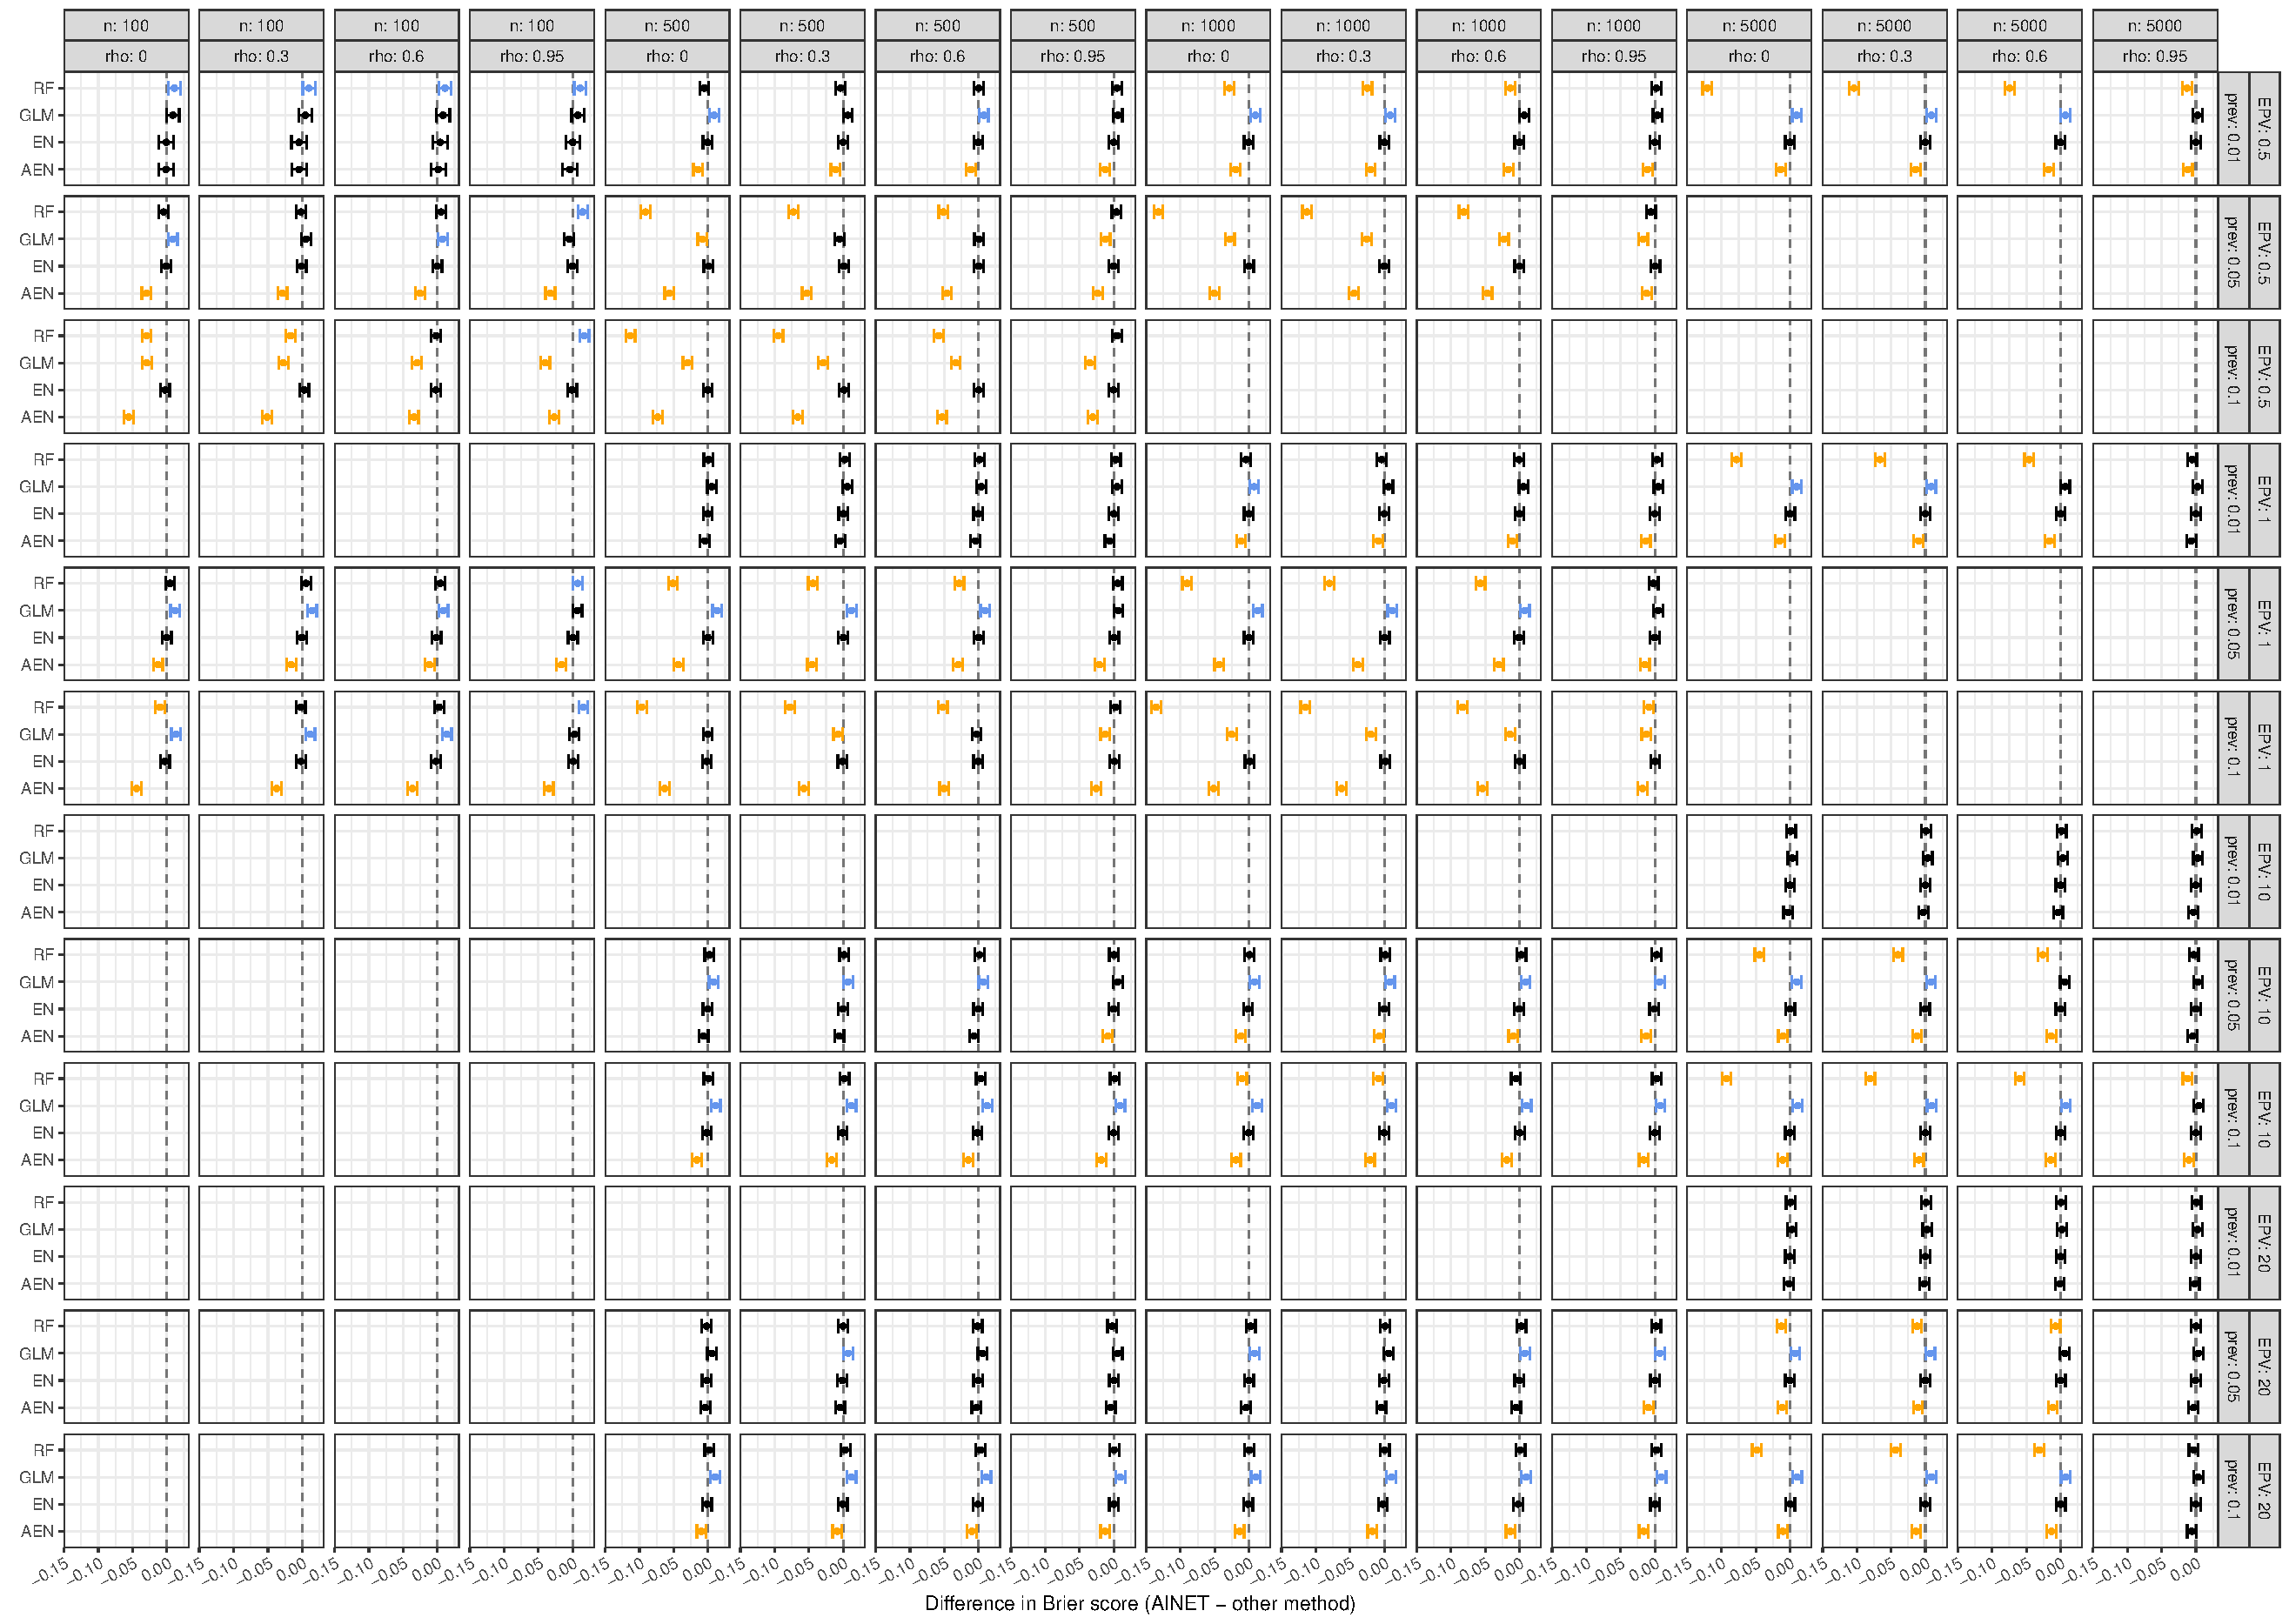
\includegraphics[width=0.9\linewidth]{figures-appendix/tie-fighter_brier.pdf}
\caption{Tie-fighter plot for the difference in Brier score between any method
  on the $y$-axis and \ainet{}. The 95\% confidence intervals are adjusted per
  simulation condition using the single-step method. Lower values indicate
  better performance of \ainet{}. } \label{fig:tiebrier}
\end{figure}
\end{landscape}
%---%---%---%---%---%---%---%---%---%---%---%---%---%---%---%---%---%---%---%---%---

%---%---%---%---%---%---%---%---%---%---%---%---%---%---%---%---%---%---%---%---%---
\begin{landscape}
\begin{figure}[!ht]
\center
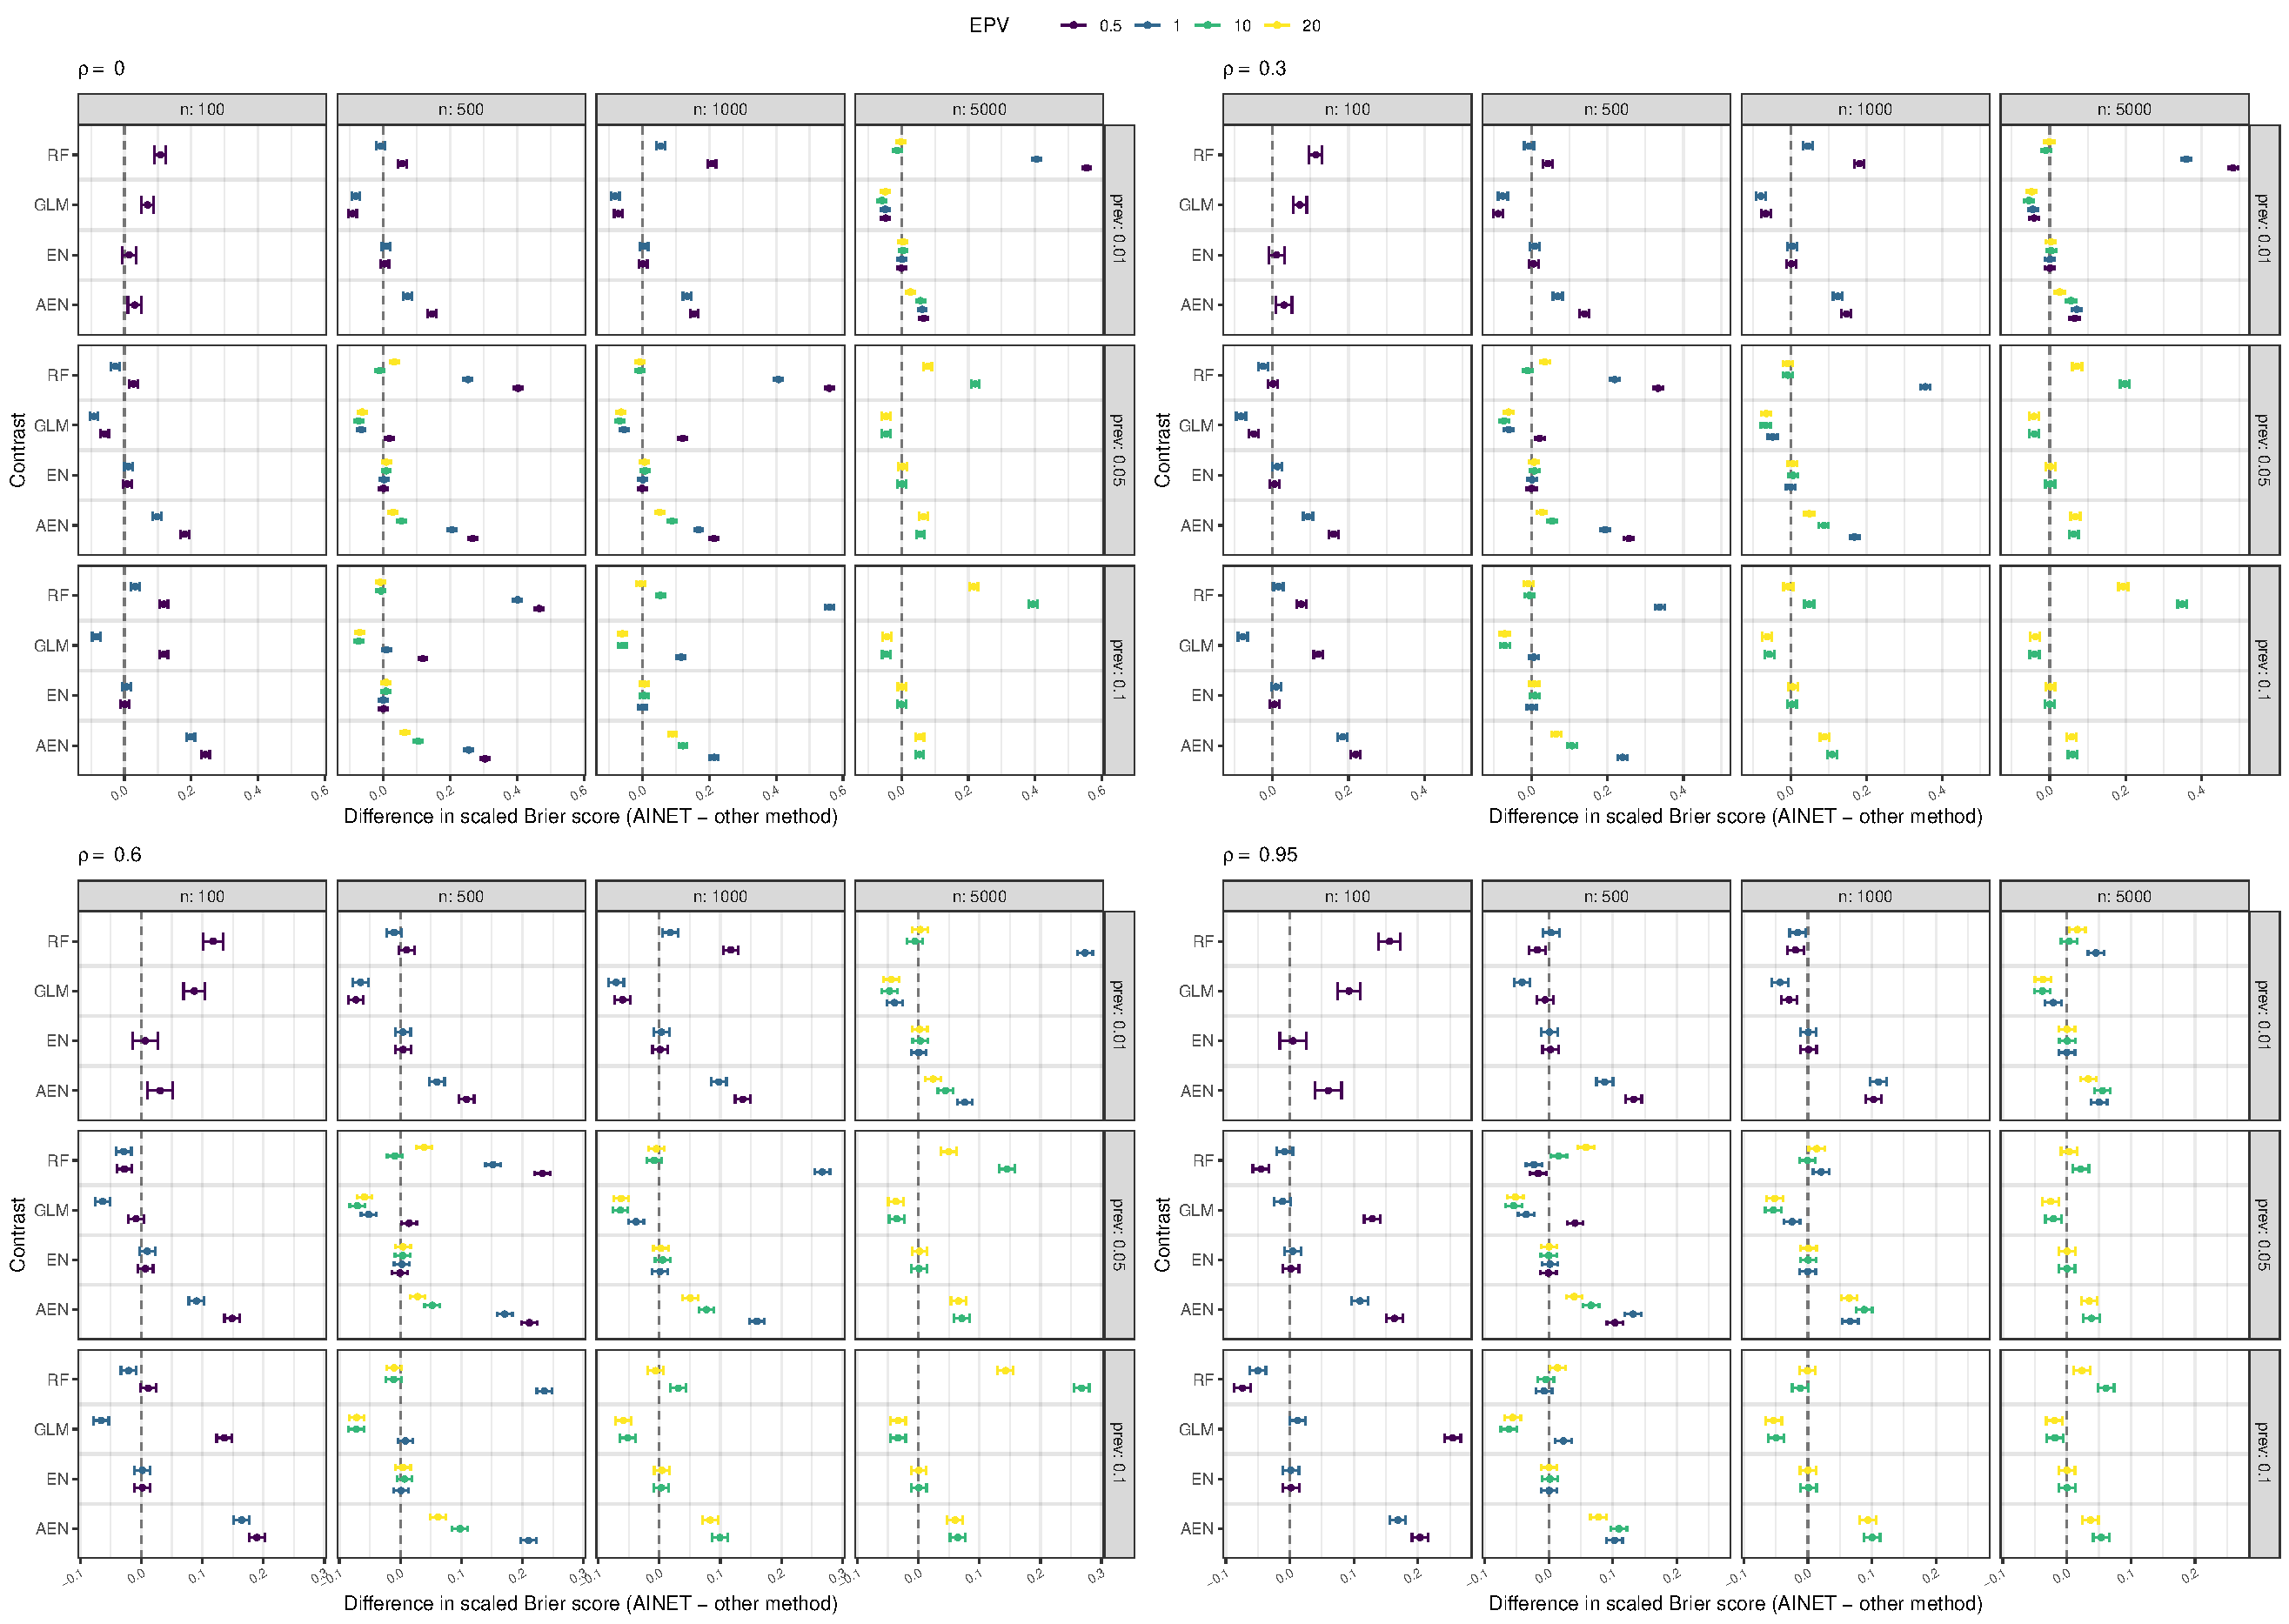
\includegraphics[width=0.9\linewidth]{figures-appendix/tie-fighter_scaledBrier.pdf}
\caption{Tie-fighter plot for the difference in scaled Brier score between any
  method on the $y$-axis and \ainet{}. The 95\% confidence intervals are adjusted
  per simulation condition using the single-step method. Larger
  values indicate better performance of \ainet{}. } \label{fig:tiesbrier}
\end{figure}
\end{landscape}
%---%---%---%---%---%---%---%---%---%---%---%---%---%---%---%---%---%---%---%---%---

%---%---%---%---%---%---%---%---%---%---%---%---%---%---%---%---%---%---%---%---%---
\begin{landscape}
\begin{figure}[!ht]
\center
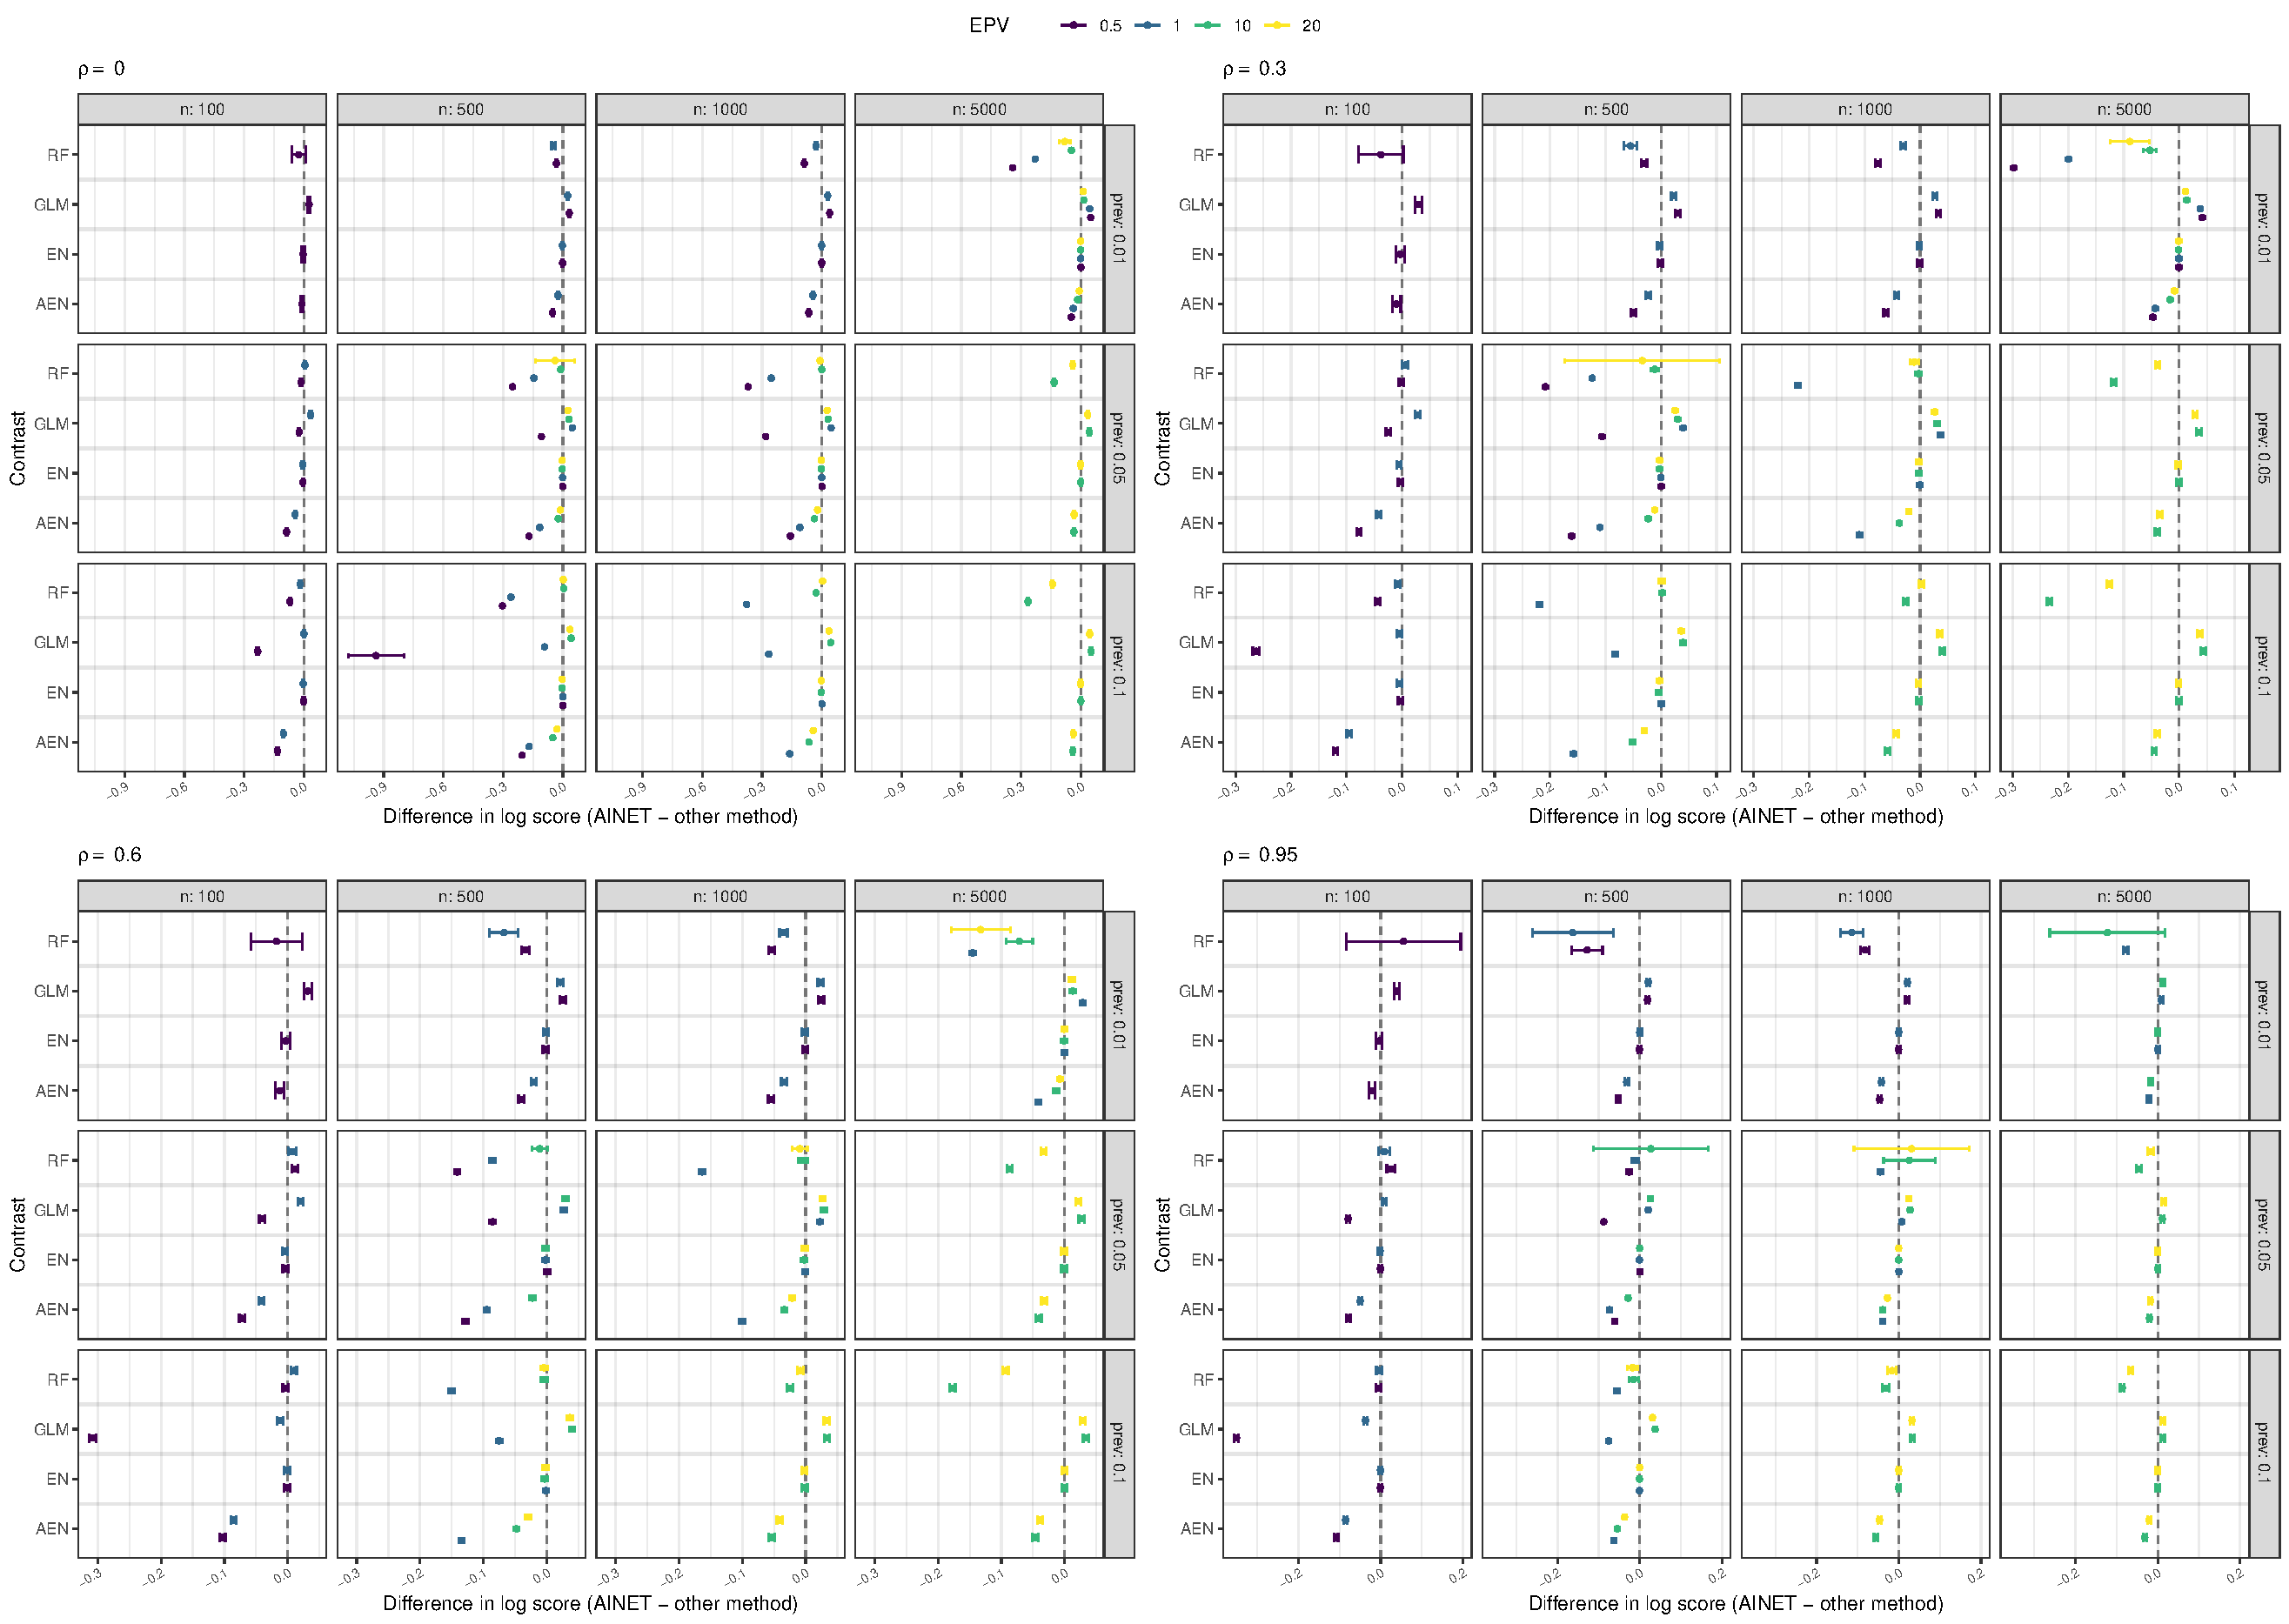
\includegraphics[width=0.9\linewidth]{figures-appendix/tie-fighter_nll.pdf}
\caption{Tie-fighter plot for the difference in log-score between any method on
  the $y$-axis and \ainet{}. The 95\% confidence intervals are adjusted per
  simulation condition using the single-step method. Lower values indicate
  better performance of \ainet{}. } \label{fig:tienll}
\end{figure}
\end{landscape}
%---%---%---%---%---%---%---%---%---%---%---%---%---%---%---%---%---%---%---%---%---

%---%---%---%---%---%---%---%---%---%---%---%---%---%---%---%---%---%---%---%---%---
\begin{landscape}
\begin{figure}[!ht]
\center
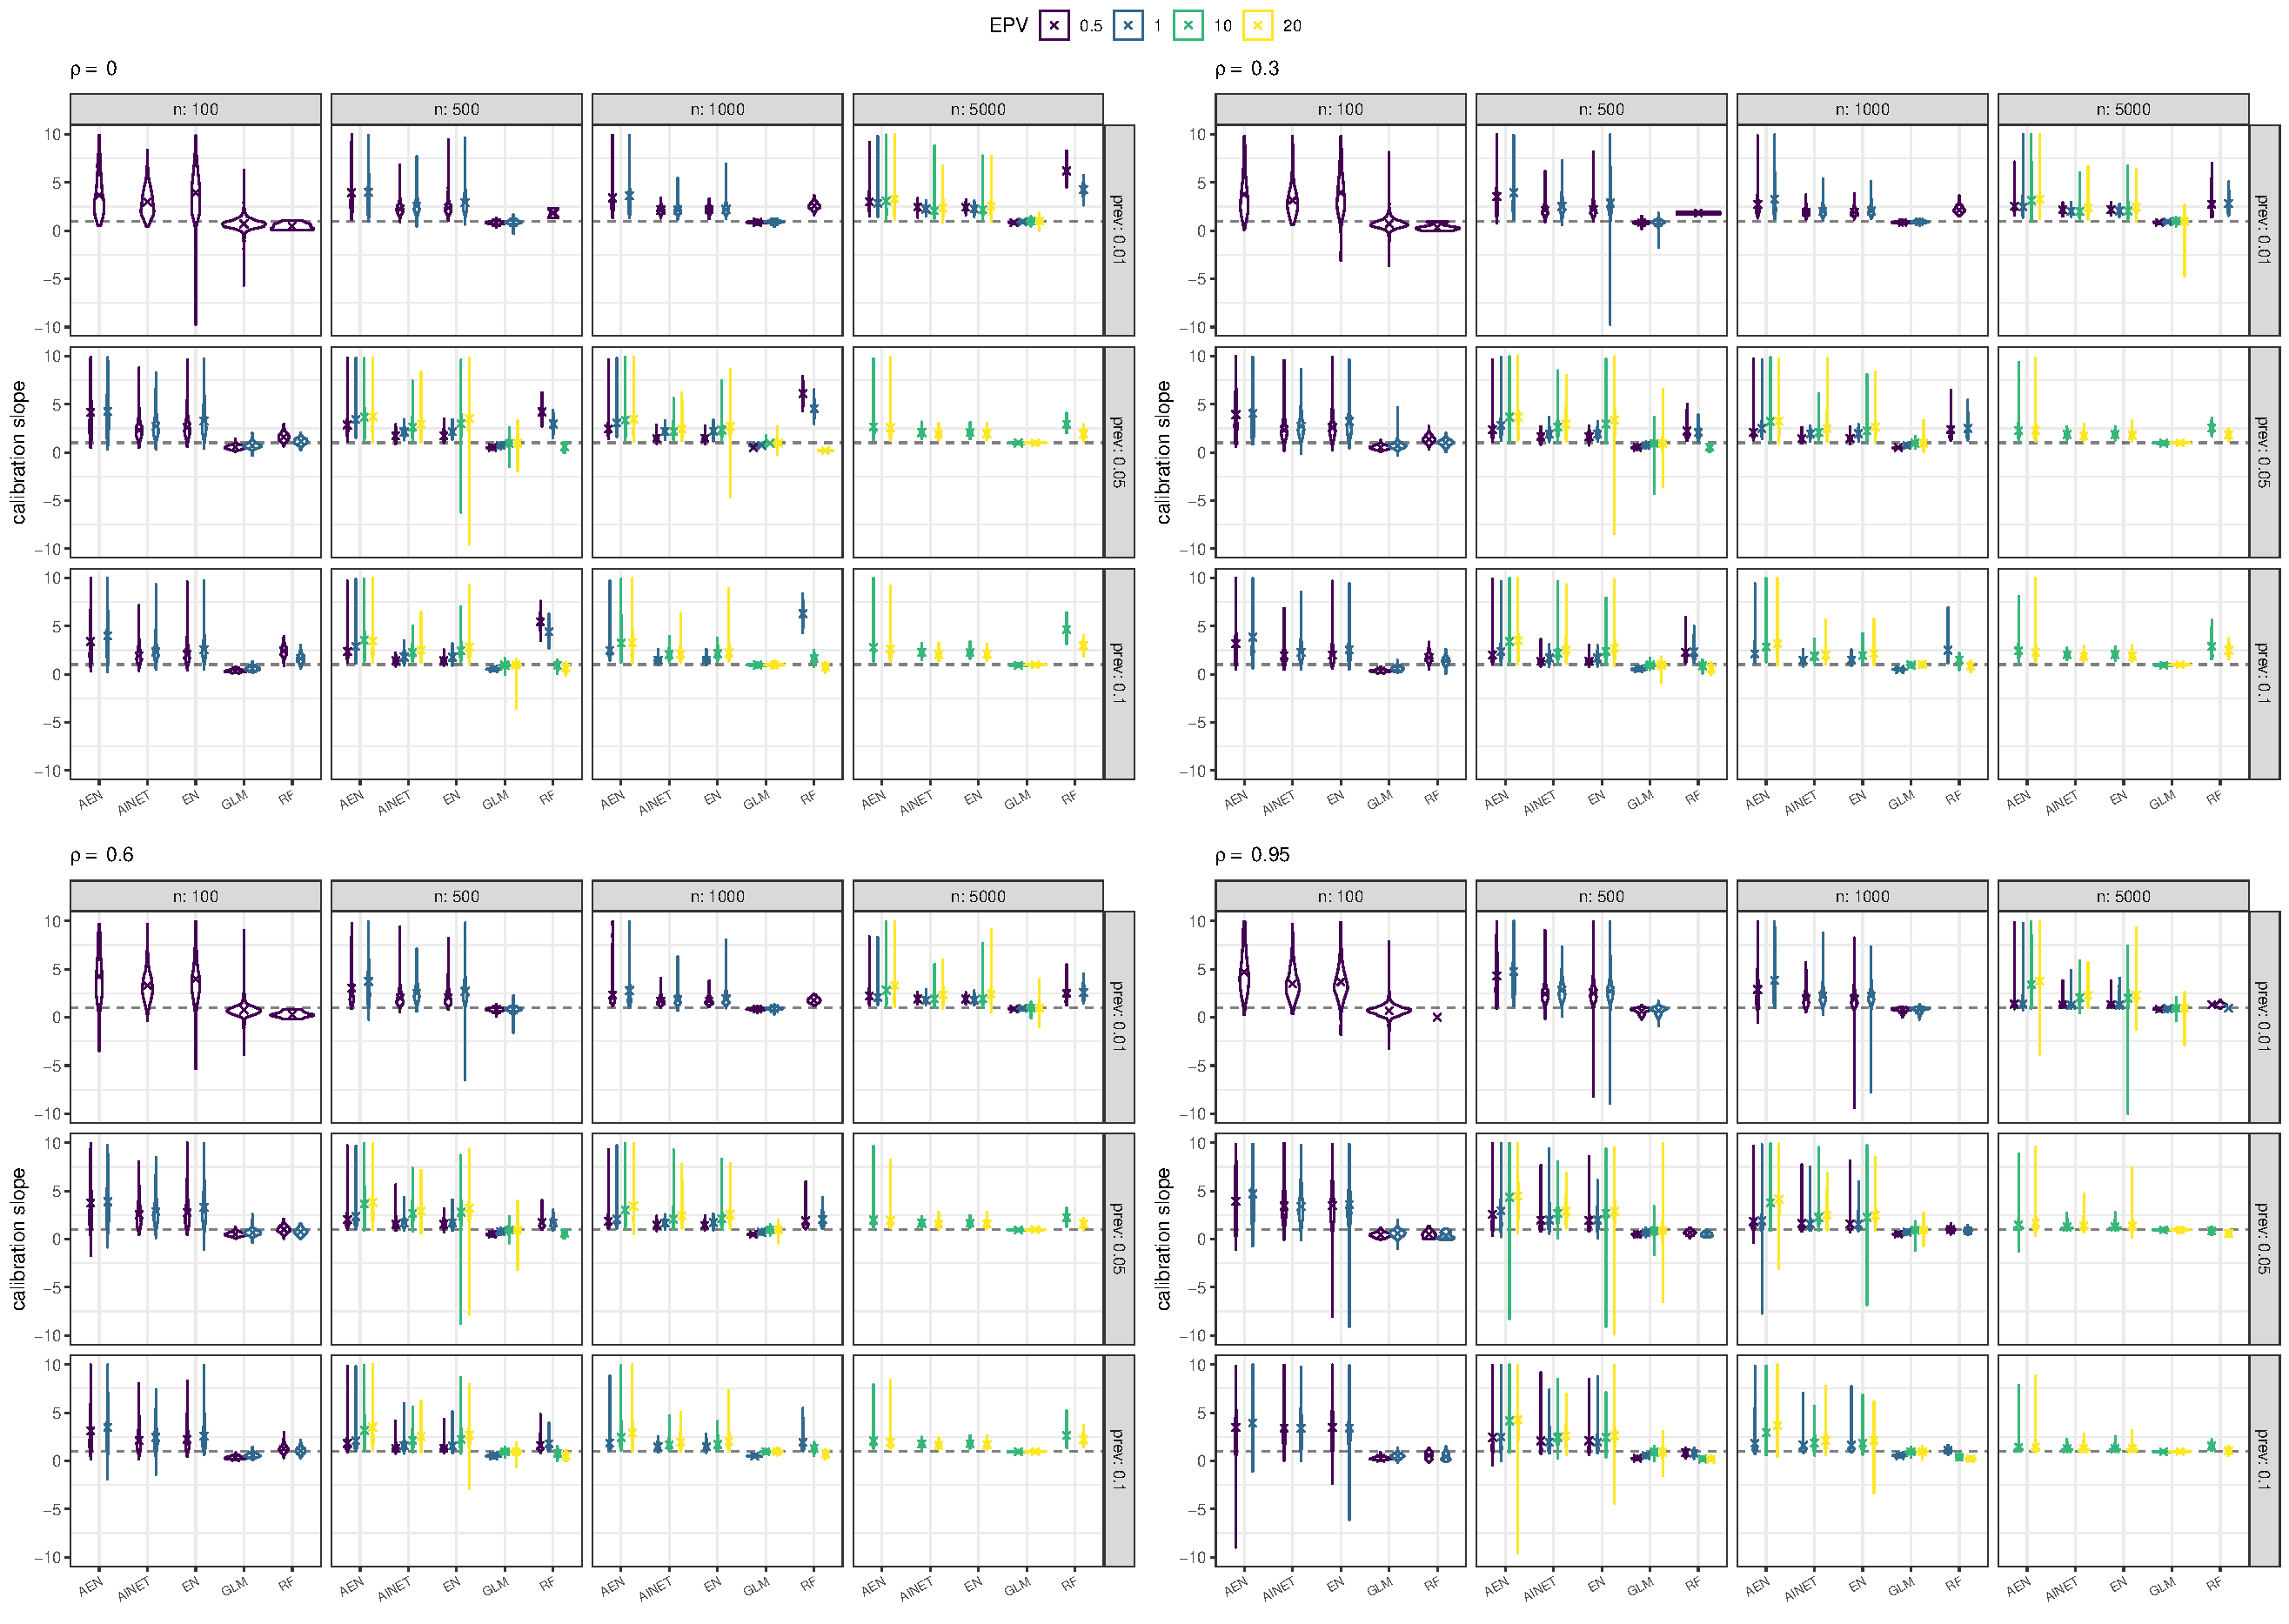
\includegraphics[width=0.9\linewidth]{figures-appendix/calibration-cslope.pdf}
\caption{Boxplots of calibration slopes stratified by method and simulation
  conditions. Mean calibration slope is indicated by a cross. A value of one
  indicates optimal calibration. Percentage of simulations where calibration
  slope could not be estimated (due to extreme predictions or complete
  separation) are also indicated.} \label{fig:cslope}
\end{figure}
\end{landscape}
%---%---%---%---%---%---%---%---%---%---%---%---%---%---%---%---%---%---%---%---%---

%---%---%---%---%---%---%---%---%---%---%---%---%---%---%---%---%---%---%---%---%---
\begin{landscape}
\begin{figure}[!ht]
\center
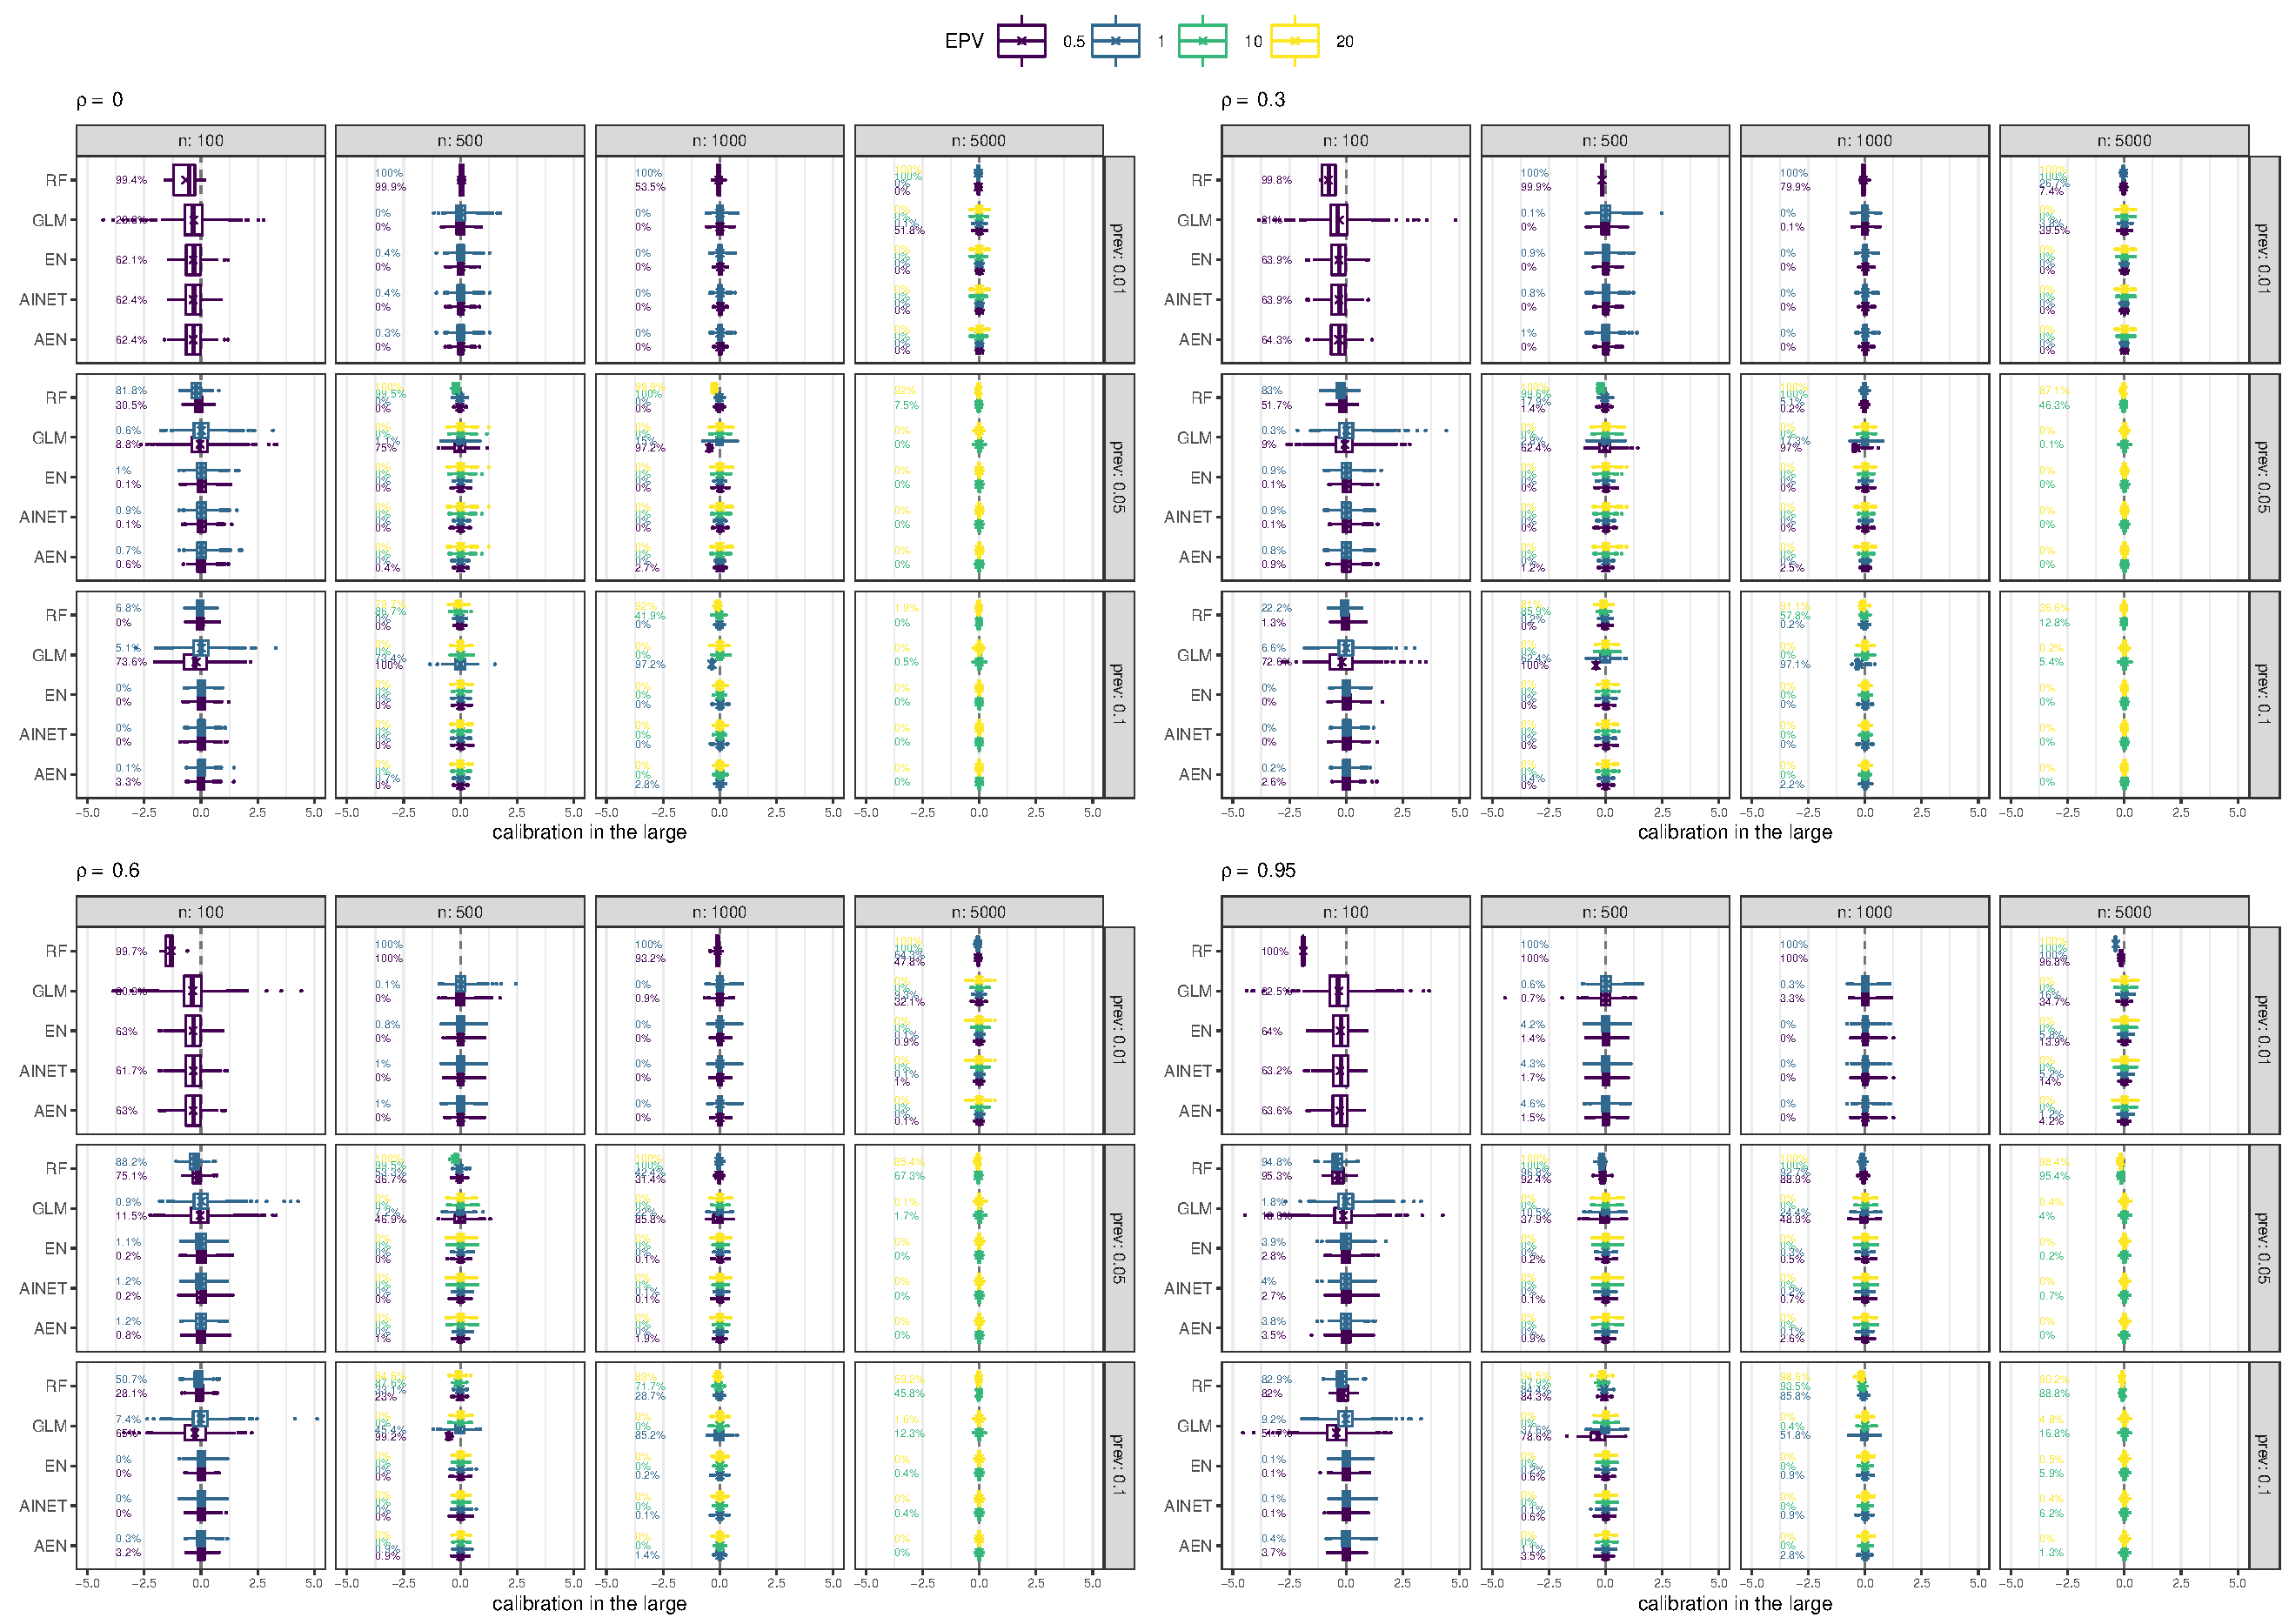
\includegraphics[width=0.9\linewidth]{figures-appendix/calibration-clarge.pdf}
\caption{Boxplots of calibration in the large stratified by method and
  simulation conditions. Mean calibration in the large is indicated by a cross.
  A value of zero indicates optimal calibration in the large. Percentage of
  simulations where calibration in the large could not be estimated (due to
  extreme predictions or complete separation) are also
  indicated.} \label{fig:clarge}
\end{figure}
\end{landscape}
%---%---%---%---%---%---%---%---%---%---%---%---%---%---%---%---%---%---%---%---%---


\end{appendices}

% Bibliography
% ======================================================================
\bibliographystyle{apalikedoiurl}
\bibliography{bibliography}

\end{document}
